\documentclass[aspectratio=169]{beamer}
\usetheme[theme=blue,logo=logowithtextvi]{HUST} 
\DeclareUnicodeCharacter{221E}{\ensuremath{\infty}}

\usepackage[T5]{fontenc}
\usepackage[utf8]{inputenc}
\usepackage{amsmath}
\usepackage{amsfonts}
\usepackage{amssymb}
\usepackage{graphicx}
\usepackage{adjustbox}
\usepackage{xcolor}
\usepackage{tikz}
\usepackage{minted}
\usepackage{tcolorbox}


\usetikzlibrary{positioning,calc,shapes.symbols,matrix,fit,backgrounds,decorations.pathreplacing,arrows.meta, shapes.geometric}
\definecolor{codeblue}{RGB}{0,90,200}   
\definecolor{codegold}{RGB}{210,160,0}
\definecolor{HUSTBlue}{RGB}{0,51,102}

\setminted{
	breaklines=false,
	autogobble=false,
	obeytabs=true,
	tabsize=2,
	linenos=true,
	showspaces=false,
	space=~,
	baselinestretch=1,
	fontsize=\normalsize,
	rulecolor=\color{black}
}

\newcommand{\placecontent}[4]{%
	\tikz[remember picture,overlay]
	\node[anchor=north west]
	at ([xshift=#1,yshift=-#2]current page.north west)
	{\parbox{#3}{#4}};
}

\graphicspath{{./week 13 resources/}}

\title{\huge CẤU TRÚC DỮ LIỆU VÀ GIẢI THUẬT}
\author{SoICT - HUST}
\date{}

\begin{document}
	
	% 2 slides đầu tiên:
	\HUSTInsertBrandSlide
	\HUSTInsertThemeSlide
	
	% Slide tiêu đề
	{\HUSTUseBackground{onelove.pdf}
		\begin{frame}
			\ifdefstring{\insertaspectratio}{169}{
				\HUSTCornerImage[0.14]{assets/logo/soict_vi_h.pdf}
				\placecontent{0.5cm}{0.33\paperheight}{0.85\paperwidth}{
					\color{\HUSTFrameTitleTextColor}\bfseries\fontsize{22pt}{30pt}\selectfont
					\inserttitle
				}
				\placecontent{0.5cm}{0.50\paperheight}{0.8\paperwidth}{
					\color{\HUSTFrameTitleTextColor}\fontsize{14pt}{14pt}\selectfont
					%Bài học
					\textbf{\large TUẦN 13: BẢNG BĂM}\\
				}
			}{}
		\end{frame}
	}
	
	% Outline
	\AtBeginSection[]
	{
		\begin{frame}<beamer>
			\frametitle{NỘI DUNG}
			\tableofcontents[currentsection]
		\end{frame}
	}
	
	%Nội dung chính trong slides
	%================== SLIDE 1 ==================%
	\begin{frame}[t]{MỤC TIÊU}
		\setlength{\leftmargini}{-1.2em}
		
		{\Large\itshape\structure{Sau bài học này, người học có thể:}}
		
		\vspace{0.8em}
		\Large
		\begin{itemize}
			\item Hiểu được ý nghĩa của \textcolor{red}{bảng băm},\\
			\textcolor{red}{hàm băm} trong việc lưu trữ và tra cứu\\
			dữ liệu
			
			\vspace{0.9em}
			\item Nắm được cách \textcolor{red}{giải quyết xung đột} khi\\
			sử dụng bảng băm
		\end{itemize}
	\end{frame}
	
	%================== SLIDE 2 ==================%
	\begin{frame}[t]{ĐẶT VẤN ĐỀ}
		\setlength{\leftmargini}{-1.2em}
		\normalsize
		
		\begin{itemize}
			\item Cho bảng $T$ và bản ghi $x$ gồm \textcolor{red}{khoá key} và \textcolor{red}{dữ liệu data} đi kèm,
			ta cần hỗ trợ các thao tác sau:
			\begin{itemize}
				\item \textcolor{red}{Insert $(T,x)$: thêm bản ghi $x(\text{key},\text{data})$ vào bảng $T$}
				\item \textcolor{red}{Delete $(T,x)$: xoá bản ghi $x(\text{key},\text{data})$ khỏi bảng $T$}
				\item \textcolor{red}{Search$(T,x)$: tìm kiếm bản ghi $x(\text{key},\text{data})$ có xuất hiện trong bảng $T$ hay không}
			\end{itemize}
			
			\item Ta muốn thực hiện các thao tác này một cách nhanh chóng mà không phải thực hiện việc sắp xếp
			các bản ghi. Bảng băm (hash table) là cách tiếp cận giải quyết vấn đề đặt ra.
			
			\item Trong bài này, ta sẽ chỉ xét khoá là các số nguyên dương (có thể rất lớn).
		\end{itemize}
	\end{frame}
	
	\section{Địa chỉ trực tiếp, bảng băm và hàm băm}
	
% (Nếu chưa có) cần: \usetikzlibrary{arrows.meta,decorations.pathmorphing}

\begin{frame}[t]{1. ĐỊA CHỈ TRỰC TIẾP, BẢNG BĂM VÀ HÀM BĂM}
	\vspace*{-0.2cm}
	\setlength{\leftmargini}{-1.2em}
	
	\begin{columns}[T,onlytextwidth]
		% LEFT: text
		\begin{column}{0.55\textwidth}
			\begin{itemize}
				\item Giả sử tập $S$ gồm $n$ phần tử, mỗi phần tử gồm khóa
				\textcolor{blue}{\textit{key}} và dữ liệu \textcolor{blue}{\textit{data}}.
				Trường khóa \textcolor{blue}{\textit{key}} của mỗi phần tử $x$:
				\begin{itemize}
					\item Là các số trong khoảng từ $0$ đến $m-1$ $(m \ge n)$
					\item Các khóa là khác nhau từng đôi.
				\end{itemize}
				
				\item Nếu sử dụng phương pháp địa chỉ trực tiếp để lưu trữ $n$ phần tử này,
				ta dùng một mảng $T[0..m-1]$:
				\begin{itemize}
					\item $T[i]=x$ nếu $x\in S$ và $\textit{key}[x]=i$
					\item $T[i]=\mathrm{NULL}$ nếu không có phần tử nào trong tập $S$
					có trường $\textit{key}=i$
				\end{itemize}
			\end{itemize}
			
			$\Rightarrow$ $T$ được gọi là bảng địa chỉ trực tiếp (\textit{direct-address table}), các phần tử trong bảng $T$ sẽ được gọi là các ô.
		\end{column}
		
		% RIGHT: figure
		\hspace*{0.5cm}
		\begin{column}{0.45\textwidth}
			\centering
			\resizebox{\linewidth}{!}{%
				\begin{tikzpicture}[x=0.9cm,y=0.9cm,>=Stealth,line cap=round,line join=round]
					\colorlet{myblue}{blue!75!black}
					
					% sizes
					\def\kw{0.45}  % key width
					\def\dw{1.20}  % data width (record)
					\def\recH{0.45}   % record height
					\def\tw{2.25}  % table width
					\def\th{4.80}  % table height
					
					% anchors
					\coordinate (Scenter) at (1.25,2.45);
					\coordinate (Tll) at (4.55,0.10);
					
					% labels
					\node[font=\scriptsize\bfseries] at ($(Scenter)+(0,2.25)$) {Tập $S$};
					\node[font=\scriptsize\bfseries] at ($(Tll)+(0.5*\tw,\th+0.75)$) {Bảng địa chỉ trực tiếp};
					\node[font=\scriptsize\bfseries] at ($(Tll)+(0.5*\tw,\th+0.35)$) {$T$};
					
					% draw set S (hand-drawn-ish ellipse)
					\draw[gray!70,line width=0.9pt]
					($(Scenter)+(-1.75,-2.00)$) .. controls ($(Scenter)+(-2.20,0.15)$) and ($(Scenter)+(-1.70,2.05)$)
					.. ($(Scenter)+(-0.10,2.10)$)
					.. controls ($(Scenter)+(1.55,2.05)$) and ($(Scenter)+(2.25,0.00)$)
					.. ($(Scenter)+(1.55,-2.05)$)
					.. controls ($(Scenter)+(0.75,-2.35)$) and ($(Scenter)+(-0.90,-2.25)$)
					.. cycle;
					
					% record helper (manual)
					% records in S
					\begin{scope}[shift={(0.55,3.35)}] % k (top)
						\draw[red,line width=1.0pt] (0,0) rectangle (\kw, \recH);
						\draw[myblue,line width=1.0pt] (\kw,0) rectangle (\kw+\dw,\recH);
						\node[font=\scriptsize\bfseries] at (0.5*\kw,0.5*\recH) {$k$};
					\end{scope}
					\begin{scope}[shift={(0.15,2.35)}] % i (middle)
						\draw[red,line width=1.0pt] (0,0) rectangle (\kw,\recH);
						\draw[myblue,line width=1.0pt] (\kw,0) rectangle (\kw+\dw,\recH);
						\node[font=\scriptsize\bfseries] at (0.5*\kw,0.5*\recH) {$i$};
					\end{scope}
					\begin{scope}[shift={(0.35,1.10)}] % j (bottom)
						\draw[red,line width=1.0pt] (0,0) rectangle (\kw,\recH);
						\draw[myblue,line width=1.0pt] (\kw,0) rectangle (\kw+\dw,\recH);
						\node[font=\scriptsize\bfseries] at (0.5*\kw,0.5*\recH) {$j$};
					\end{scope}
					
					% table T outline + dashed split
					\draw[gray!70,line width=0.9pt] (Tll) rectangle ++(\tw,\th);
					\draw[gray!70,dashed,line width=0.8pt] ($(Tll)+(\kw,0)$) -- ($(Tll)+(\kw,\th)$);
					
					% occupied slots (i, j, k)
					\def\yi{3.55}
					\def\yj{2.70}
					\def\yk{1.15}
					
					\foreach \lab/\yy in {i/\yi, j/\yj, k/\yk}{
						\draw[red,line width=1.0pt] ($(Tll)+(0,\yy)$) rectangle ++(\kw,\recH);
						\draw[myblue,line width=1.0pt] ($(Tll)+(\kw,\yy)$) rectangle ++(\tw-\kw,\recH);
						\node[font=\scriptsize\bfseries] at ($(Tll)+(0.5*\kw,\yy+0.5*\recH)$) {$\lab$};
						\node[font=\scriptsize] at ($(Tll)+(\tw+0.25,\yy+0.5*\recH)$) {$\lab$};
					}
					
					% m arrow (height)
					\draw[<->,line width=0.9pt] ($(Tll)+(\tw+0.70,0)$) -- ($(Tll)+(\tw+0.70,\th)$);
					\node[font=\scriptsize, xshift=7pt] at ($(Tll)+(\tw+0.70,0.5*\th)$) {$m$};
					
					% red arrows from S to T
					\draw[->,red,very thick]
					(0.15+\kw+\dw,2.35+0.5*\recH) -- ($(Tll)+(0,\yi+0.5*\recH)$);
					
					\draw[->,red,very thick]
					(0.35+\kw+\dw,1.10+0.5*\recH)
					.. controls (2.25,1.75) and (3.15,2.55) ..
					($(Tll)+(0,\yj+0.5*\recH)$);
					
					\draw[->,red,very thick]
					(0.55+\kw+\dw,3.35+0.5*\recH)
					.. controls (2.35,3.05) and (3.20,1.80) ..
					($(Tll)+(0,\yk+0.5*\recH)$);
					
			\end{tikzpicture}}
		\end{column}
	\end{columns}
\end{frame}

% ===== SLIDE 9 =====
\begin{frame}[t]{1. ĐỊA CHỈ TRỰC TIẾP, BẢNG BĂM VÀ HÀM BĂM}
	\setlength{\leftmargini}{-1.2em}
	\vspace*{-0.3cm}
	
	\begin{columns}[T,onlytextwidth]
		% LEFT
		\begin{column}{0.55\textwidth}
			\begin{itemize}
				\item Nếu sử dụng phương pháp địa chỉ trực tiếp để lưu trữ $n$ phần tử này, ta dùng một mảng $T[0..m-1]$:
				\begin{itemize}
					\item $T[i]=x$ nếu $x\in S$ và $key[x]=i$
					\item $T[i]=\mathrm{NULL}$ nếu không có phần tử nào trong tập $S$ có trường $key=i$
				\end{itemize}
				\item Các phép toán được cài đặt một cách trực tiếp:
				\begin{itemize}
					\item \textcolor{red}{SEARCH$(T,k)$}\\[-0.2em]
					\textbf{return} $T[k]$
					
					\vspace{0.5em}
					\item \textcolor{red}{INSERT$(T,x)$}\\[-0.2em]
					$T[key[x]] = x$
					
					\vspace{0.5em}
					\item \textcolor{red}{DELETE$(T,x)$}\\[-0.2em]
					$T[key[x]] = \mathrm{NULL}$
				\end{itemize}
			\end{itemize}
			Thời gian thực hiện mỗi phép toán đều là $O(1)$.
		\end{column}
		
		% RIGHT
		\hspace*{0.5cm}
		\begin{column}{0.45\textwidth}
			\centering
			\vspace{0.2em}
			\resizebox{0.98\linewidth}{!}{%
				\begin{tikzpicture}[x=0.9cm,y=0.9cm,>=Stealth,line cap=round,line join=round]
					\colorlet{myblue}{blue!75!black}
					
					% sizes
					\def\kw{0.45}  % key width
					\def\dw{1.20}  % data width (record)
					\def\recH{0.45}   % record height
					\def\tw{2.25}  % table width
					\def\th{4.80}  % table height
					
					% anchors
					\coordinate (Scenter) at (1.25,2.45);
					\coordinate (Tll) at (4.55,0.10);
					
					% labels
					\node[font=\scriptsize\bfseries] at ($(Scenter)+(0,2.25)$) {Tập $S$};
					\node[font=\scriptsize\bfseries] at ($(Tll)+(0.5*\tw,\th+0.75)$) {Bảng địa chỉ trực tiếp};
					\node[font=\scriptsize\bfseries] at ($(Tll)+(0.5*\tw,\th+0.35)$) {$T$};
					
					% draw set S (hand-drawn-ish ellipse)
					\draw[gray!70,line width=0.9pt]
					($(Scenter)+(-1.75,-2.00)$) .. controls ($(Scenter)+(-2.20,0.15)$) and ($(Scenter)+(-1.70,2.05)$)
					.. ($(Scenter)+(-0.10,2.10)$)
					.. controls ($(Scenter)+(1.55,2.05)$) and ($(Scenter)+(2.25,0.00)$)
					.. ($(Scenter)+(1.55,-2.05)$)
					.. controls ($(Scenter)+(0.75,-2.35)$) and ($(Scenter)+(-0.90,-2.25)$)
					.. cycle;
					
					% records in S
					\begin{scope}[shift={(0.55,3.35)}] % k (top)
						\draw[red,line width=1.0pt] (0,0) rectangle (\kw,\recH);
						\draw[myblue,line width=1.0pt] (\kw,0) rectangle (\kw+\dw,\recH);
						\node[font=\scriptsize\bfseries] at (0.5*\kw,0.5*\recH) {$k$};
					\end{scope}
					\begin{scope}[shift={(0.15,2.35)}] % i (middle)
						\draw[red,line width=1.0pt] (0,0) rectangle (\kw,\recH);
						\draw[myblue,line width=1.0pt] (\kw,0) rectangle (\kw+\dw,\recH);
						\node[font=\scriptsize\bfseries] at (0.5*\kw,0.5*\recH) {$i$};
					\end{scope}
					\begin{scope}[shift={(0.35,1.10)}] % j (bottom)
						\draw[red,line width=1.0pt] (0,0) rectangle (\kw,\recH);
						\draw[myblue,line width=1.0pt] (\kw,0) rectangle (\kw+\dw,\recH);
						\node[font=\scriptsize\bfseries] at (0.5*\kw,0.5*\recH) {$j$};
					\end{scope}
					
					% table T outline + dashed split
					\draw[gray!70,line width=0.9pt] (Tll) rectangle ++(\tw,\th);
					\draw[gray!70,dashed,line width=0.8pt] ($(Tll)+(\kw,0)$) -- ($(Tll)+(\kw,\th)$);
					
					% occupied slots (i, j, k)
					\def\yi{3.55}
					\def\yj{2.70}
					\def\yk{1.15}
					
					\foreach \lab/\yy in {i/\yi, j/\yj, k/\yk}{
						\draw[red,line width=1.0pt] ($(Tll)+(0,\yy)$) rectangle ++(\kw,\recH);
						\draw[myblue,line width=1.0pt] ($(Tll)+(\kw,\yy)$) rectangle ++(\tw-\kw,\recH);
						\node[font=\scriptsize\bfseries] at ($(Tll)+(0.5*\kw,\yy+0.5*\recH)$) {$\lab$};
						\node[font=\scriptsize] at ($(Tll)+(\tw+0.25,\yy+0.5*\recH)$) {$\lab$};
					}
					
					% m arrow (height)
					\draw[<->,line width=0.9pt] ($(Tll)+(\tw+0.70,0)$) -- ($(Tll)+(\tw+0.70,\th)$);
					\node[font=\scriptsize, xshift=7pt] at ($(Tll)+(\tw+0.70,0.5*\th)$) {$m$};
					
					% red arrows from S to T
					\draw[->,red,very thick]
					(0.15+\kw+\dw,2.35+0.5*\recH) -- ($(Tll)+(0,\yi+0.5*\recH)$);
					
					\draw[->,red,very thick]
					(0.35+\kw+\dw,1.10+0.5*\recH)
					.. controls (2.25,1.75) and (3.15,2.5) ..
					($(Tll)+(0,\yj+0.5*\recH)$);
					
					\draw[->,red,very thick]
					(0.55+\kw+\dw,3.35+0.5*\recH)
					.. controls (2.35,3.05) and (3.20,1.80) ..
					($(Tll)+(0,\yk+0.5*\recH)$);
				\end{tikzpicture}%
			}
		\end{column}
	\end{columns}
\end{frame}


% ===== SLIDE 10 =====
\begin{frame}[t]{1. ĐỊA CHỈ TRỰC TIẾP, BẢNG BĂM VÀ HÀM BĂM}
	\setlength{\leftmargini}{-1.2em}
	
	\begin{itemize}
		\item Hạn chế của phương pháp địa chỉ trực tiếp:
		\begin{itemize}
			\item Tốn bộ nhớ khi: số phần tử $n \ll m$ (Phương pháp địa chỉ trực tiếp làm việc tốt nếu như biên
			độ $m$ của các khóa là tương đối nhỏ).
			\item Nếu các khoá là các số nguyên 32-bit thì sao?
			\begin{itemize}
				\item Vấn đề 1: bảng địa chỉ trực tiếp sẽ phải có $2^{32}$ (hơn 4 tỷ) phần tử
				\item Vấn đề 2: ngay cả khi bộ nhớ không là vấn đề, thì thời gian khởi tạo các phần tử là
				\texttt{NULL} cũng là rất tốn kém
			\end{itemize}
		\end{itemize}
		
		\vspace{0.6em}
		\item Cách giải quyết: Ánh xạ khoá từ khoảng $0..m-1$ vào khoảng biến đổi nhỏ hơn.
	\end{itemize}
	
	\vspace{0.8em}
	$\Rightarrow$ Ánh xạ này được gọi là hàm băm (\textit{hash function}) và bảng lưu trữ lúc này được gọi là bảng băm
	(\textit{hash table}).
\end{frame}

%--- Slide: Địa chỉ trực tiếp, bảng băm và hàm băm
\begin{frame}[t]{1. ĐỊA CHỈ TRỰC TIẾP, BẢNG BĂM VÀ HÀM BĂM}
	\small
	\vspace*{-0.3cm}
	\setlength{\leftmargini}{-1.2em}
	
	\begin{columns}[T,onlytextwidth]
		%================ LEFT =================
		\begin{column}{0.60\textwidth}
			\begin{itemize}
				\item Trong phương pháp địa chỉ trực tiếp, phần tử với khoá $k$ được cất giữ ở ô $k$.
				
				\item Với bảng băm, phần tử với khoá $k$ được cất giữ ở ô $h(k)$, trong đó ta sử dụng hàm băm $h$
				để xác định ô cất giữ phần tử này từ khoá của nó $(k)$.
				
				\item \textcolor{red}{\textit{Định nghĩa.} Hàm băm $h$ là ánh xạ từ không gian khoá $U$ vào các ô của bảng băm $T[0..p-1]$:}
				
				\hspace{2.5cm}\color{red}$h: U \rightarrow \{0,\,1,\,\ldots,\,p-1\}$
					
				\begin{itemize}
					\item[$\bullet$] Ta sẽ nói rằng phần tử với khoá $k$ được gắn vào ô $h(k)$,
					và nói $h(k)$ là giá trị băm của khoá $k$.
				\end{itemize}
			\end{itemize}
			
			$\Rightarrow$ Vấn đề nảy sinh lại là xung đột (\textit{collision}), khi nhiều khoá được đặt tương ứng
			với cùng một ô trong bảng địa chỉ $T$.
		\end{column}
		
		%================ RIGHT =================
		\begin{column}{0.32\textwidth}
			\centering
			\vspace*{1cm}
			
			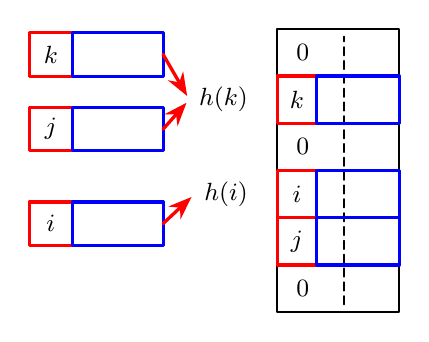
\begin{tikzpicture}[
				x=1cm,y=1cm,
				>=Stealth,
				line cap=round,line join=round,
				font=\small
				]
				%----- parameters
				\def\rowH{0.60}
				\def\nrow{6}
				\def\tw{1.55}        % table width
				\def\th{3.60}        % table height = 6*0.6
				\def\keyW{0.50}      % red key cell width (in table)
				\def\valW{1.05}      % blue cell width  (in table)
				\def\dashX{0.85}     % dashed vertical line position
				
				% table bottom-left
				\coordinate (TBL) at (3.35,0.00);
				
				%----- draw table outer + row separators
				\draw[black, line width=0.8pt] (TBL) rectangle ++(\tw,\th);
				\foreach \r in {1,2,3,4,5}{
					\draw[black, line width=0.6pt]
					($(TBL)+(0,\r*\rowH)$) -- ($(TBL)+(\tw,\r*\rowH)$);
				}
				
				% dashed vertical line (inside table)
				\draw[black, densely dashed, line width=0.7pt]
				($(TBL)+(\dashX,0.10)$) -- ($(TBL)+(\dashX,\th-0.10)$);
				
				%----- place 0's
				\node[anchor=west] at ($(TBL)+(0.12,5*\rowH+0.30)$) {$0$}; % top
				\node[anchor=west] at ($(TBL)+(0.12,3*\rowH+0.30)$) {$0$}; % middle
				\node[anchor=west] at ($(TBL)+(0.12,0*\rowH+0.30)$) {$0$}; % bottom
				
				%----- colored rows: k at row4, i at row2, j at row1
				% row4: k
				\draw[red,  line width=1.1pt] ($(TBL)+(0,4*\rowH)$) rectangle ++(\keyW,\rowH);
				\draw[blue, line width=1.1pt] ($(TBL)+(\keyW,4*\rowH)$) rectangle ++(\valW,\rowH);
				\node at ($(TBL)+(\keyW/2,4*\rowH+0.30)$) {$k$};
				
				% row2: i
				\draw[red,  line width=1.1pt] ($(TBL)+(0,2*\rowH)$) rectangle ++(\keyW,\rowH);
				\draw[blue, line width=1.1pt] ($(TBL)+(\keyW,2*\rowH)$) rectangle ++(\valW,\rowH);
				\node at ($(TBL)+(\keyW/2,2*\rowH+0.30)$) {$i$};
				
				% row1: j
				\draw[red,  line width=1.1pt] ($(TBL)+(0,1*\rowH)$) rectangle ++(\keyW,\rowH);
				\draw[blue, line width=1.1pt] ($(TBL)+(\keyW,1*\rowH)$) rectangle ++(\valW,\rowH);
				\node at ($(TBL)+(\keyW/2,1*\rowH+0.30)$) {$j$};
				
				%===== nhãn h(k), h(i) (mũi tên sẽ CHỈ VÀO CHỮ)
				\coordinate (hkLbl) at ($(TBL)+(-0.25,4*\rowH+0.30)$);
				\node[anchor=east] (hkNode) at (hkLbl) {$h(k)$};
				
				\coordinate (hiLbl) at ($(TBL)+(-0.25,2*\rowH+0.30)$);
				\node[anchor=east] (hiNode) at (hiLbl) {$h(i)$};
				
				%----- key boxes on the left (k, j, i)
				\def\bxX{0.20}
				\def\bxRedW{0.55}
				\def\bxBlueW{1.15}
				\def\bxH{0.55}
				
				% top: k
				\coordinate (B1) at (\bxX,3.00);
				\draw[red,  line width=1.1pt] (B1) rectangle ++(\bxRedW,\bxH);
				\draw[blue, line width=1.1pt] ($(B1)+(\bxRedW,0)$) rectangle ++(\bxBlueW,\bxH);
				\node at ($(B1)+(\bxRedW/2,\bxH/2)$) {$k$};
				\coordinate (kSrc) at ($(B1)+(\bxRedW+\bxBlueW, \bxH/2)$);
				
				% middle: j
				\coordinate (B2) at (\bxX,2.05);
				\draw[red,  line width=1.1pt] (B2) rectangle ++(\bxRedW,\bxH);
				\draw[blue, line width=1.1pt] ($(B2)+(\bxRedW,0)$) rectangle ++(\bxBlueW,\bxH);
				\node at ($(B2)+(\bxRedW/2,\bxH/2)$) {$j$};
				\coordinate (jSrc) at ($(B2)+(\bxRedW+\bxBlueW, \bxH/2)$);
				
				% bottom: i
				\coordinate (B3) at (\bxX,0.85);
				\draw[red,  line width=1.1pt] (B3) rectangle ++(\bxRedW,\bxH);
				\draw[blue, line width=1.1pt] ($(B3)+(\bxRedW,0)$) rectangle ++(\bxBlueW,\bxH);
				\node at ($(B3)+(\bxRedW/2,\bxH/2)$) {$i$};
				\coordinate (iSrc) at ($(B3)+(\bxRedW+\bxBlueW, \bxH/2)$);
				
				%----- red arrows: CHỈ VÀO CHỮ h(k), h(i)
				\draw[->, red, line width=1.2pt, shorten >=1.5pt] (kSrc) -- (hkNode.west);
				\draw[->, red, line width=1.2pt, shorten >=1.5pt] (jSrc) -- (hkNode.west);
				\draw[->, red, line width=1.2pt, shorten >=1.5pt] (iSrc) -- (hiNode.west);
				
			\end{tikzpicture}
			
			
		\end{column}
	\end{columns}
\end{frame}

\section{Xung đột và giải quyết xung đột}

\begin{frame}[t]{2. XUNG ĐỘT VÀ GIẢI QUYẾT XUNG ĐỘT}
	\small
	\setlength{\leftmargini}{-1.2em}
	
	\begin{columns}[T,onlytextwidth]
		%================ LEFT =================
		\begin{column}{0.60\textwidth}
			\begin{itemize}
				\item Xung đột (\textit{collision}): xảy ra khi nhiều khoá được đặt tương ứng
				với cùng một ô trong bảng băm $T$.
				
				\item \textit{Ta cần giải quyết xung đột như thế nào?}
				\begin{itemize}
					\item Cách giải quyết 1:
					\vspace{0.35em}
					
					{\color{red}\textit{Tạo chuỗi (chaining)}}
					
					\vspace{0.55em}
					\item Cách giải quyết 2:
					\vspace{0.35em}
					
					{\color{red}\textit{Phương pháp địa chỉ mở (open addressing)}}
				\end{itemize}
			\end{itemize}
		\end{column}
		
		%================ RIGHT =================
		\begin{column}{0.36\textwidth}
			\centering
			\vspace{1cm}
			\resizebox{0.95\linewidth}{!}{%
				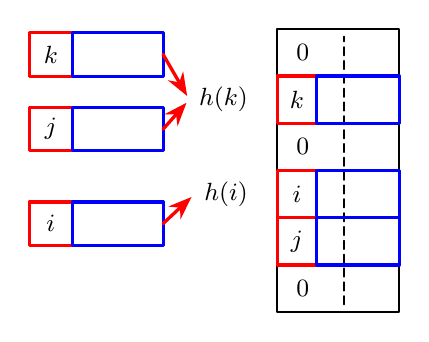
\begin{tikzpicture}[
					x=1cm,y=1cm,
					>=Stealth,
					line cap=round,line join=round,
					font=\small
					]
					%----- parameters
					\def\rowH{0.60}
					\def\nrow{6}
					\def\tw{1.55}        % table width
					\def\th{3.60}        % table height = 6*0.6
					\def\keyW{0.50}      % red key cell width (in table)
					\def\valW{1.05}      % blue cell width  (in table)
					\def\dashX{0.85}     % dashed vertical line position
					
					% table bottom-left
					\coordinate (TBL) at (3.35,0.00);
					
					%----- draw table outer + row separators
					\draw[black, line width=0.8pt] (TBL) rectangle ++(\tw,\th);
					\foreach \r in {1,2,3,4,5}{
						\draw[black, line width=0.6pt]
						($(TBL)+(0,\r*\rowH)$) -- ($(TBL)+(\tw,\r*\rowH)$);
					}
					
					% dashed vertical line (inside table)
					\draw[black, densely dashed, line width=0.7pt]
					($(TBL)+(\dashX,0.10)$) -- ($(TBL)+(\dashX,\th-0.10)$);
					
					%----- place 0's
					\node[anchor=west] at ($(TBL)+(0.12,5*\rowH+0.30)$) {$0$}; % top
					\node[anchor=west] at ($(TBL)+(0.12,3*\rowH+0.30)$) {$0$}; % middle
					\node[anchor=west] at ($(TBL)+(0.12,0*\rowH+0.30)$) {$0$}; % bottom
					
					%----- colored rows: k at row4, i at row2, j at row1
					% row4: k
					\draw[red,  line width=1.1pt] ($(TBL)+(0,4*\rowH)$) rectangle ++(\keyW,\rowH);
					\draw[blue, line width=1.1pt] ($(TBL)+(\keyW,4*\rowH)$) rectangle ++(\valW,\rowH);
					\node at ($(TBL)+(\keyW/2,4*\rowH+0.30)$) {$k$};
					
					% row2: i
					\draw[red,  line width=1.1pt] ($(TBL)+(0,2*\rowH)$) rectangle ++(\keyW,\rowH);
					\draw[blue, line width=1.1pt] ($(TBL)+(\keyW,2*\rowH)$) rectangle ++(\valW,\rowH);
					\node at ($(TBL)+(\keyW/2,2*\rowH+0.30)$) {$i$};
					
					% row1: j
					\draw[red,  line width=1.1pt] ($(TBL)+(0,1*\rowH)$) rectangle ++(\keyW,\rowH);
					\draw[blue, line width=1.1pt] ($(TBL)+(\keyW,1*\rowH)$) rectangle ++(\valW,\rowH);
					\node at ($(TBL)+(\keyW/2,1*\rowH+0.30)$) {$j$};
					
					%===== labels h(k), h(i): arrows point to the TEXT
					\coordinate (hkLbl) at ($(TBL)+(-0.25,4*\rowH+0.30)$);
					\node[anchor=east] (hkNode) at (hkLbl) {$h(k)$};
					
					\coordinate (hiLbl) at ($(TBL)+(-0.25,2*\rowH+0.30)$);
					\node[anchor=east] (hiNode) at (hiLbl) {$h(i)$};
					
					%----- key boxes on the left (k, j, i)
					\def\bxX{0.20}
					\def\bxRedW{0.55}
					\def\bxBlueW{1.15}
					\def\bxH{0.55}
					
					% top: k
					\coordinate (B1) at (\bxX,3.00);
					\draw[red,  line width=1.1pt] (B1) rectangle ++(\bxRedW,\bxH);
					\draw[blue, line width=1.1pt] ($(B1)+(\bxRedW,0)$) rectangle ++(\bxBlueW,\bxH);
					\node at ($(B1)+(\bxRedW/2,\bxH/2)$) {$k$};
					\coordinate (kSrc) at ($(B1)+(\bxRedW+\bxBlueW, \bxH/2)$);
					
					% middle: j
					\coordinate (B2) at (\bxX,2.05);
					\draw[red,  line width=1.1pt] (B2) rectangle ++(\bxRedW,\bxH);
					\draw[blue, line width=1.1pt] ($(B2)+(\bxRedW,0)$) rectangle ++(\bxBlueW,\bxH);
					\node at ($(B2)+(\bxRedW/2,\bxH/2)$) {$j$};
					\coordinate (jSrc) at ($(B2)+(\bxRedW+\bxBlueW, \bxH/2)$);
					
					% bottom: i
					\coordinate (B3) at (\bxX,0.85);
					\draw[red,  line width=1.1pt] (B3) rectangle ++(\bxRedW,\bxH);
					\draw[blue, line width=1.1pt] ($(B3)+(\bxRedW,0)$) rectangle ++(\bxBlueW,\bxH);
					\node at ($(B3)+(\bxRedW/2,\bxH/2)$) {$i$};
					\coordinate (iSrc) at ($(B3)+(\bxRedW+\bxBlueW, \bxH/2)$);
					
					%----- red arrows: point to the TEXT h(k), h(i)
					\draw[->, red, line width=1.2pt, shorten >=1.5pt] (kSrc) -- (hkNode.west);
					\draw[->, red, line width=1.2pt, shorten >=1.5pt] (jSrc) -- (hkNode.west);
					\draw[->, red, line width=1.2pt, shorten >=1.5pt] (iSrc) -- (hiNode.west);
					
				\end{tikzpicture}%
			}
		\end{column}
	\end{columns}
\end{frame}

% --- SLIDE: Xung đột và giải quyết xung đột (tạo chuỗi / chaining)
\begin{frame}[t]{2. XUNG ĐỘT VÀ GIẢI QUYẾT XUNG ĐỘT}
	\small
	\setlength{\leftmargini}{-1.2em}
	
	\begin{itemize}
		\item Cách giải quyết xung đột bằng \textcolor{red}{phương pháp tạo chuỗi}:
		\begin{itemize}
			\item Tạo danh sách liên kết để chứa các phần tử được gắn với cùng một vị trí trong bảng.
			Ví dụ: $h(k)=k \bmod p$. Nếu ô $T[h(k)]$ trong bảng băm đã bận, ta thêm phần tử mới này vào
			đầu danh sách móc nối tại ô $T[h(k)]$.
		\end{itemize}
	\end{itemize}
	
	\centering
	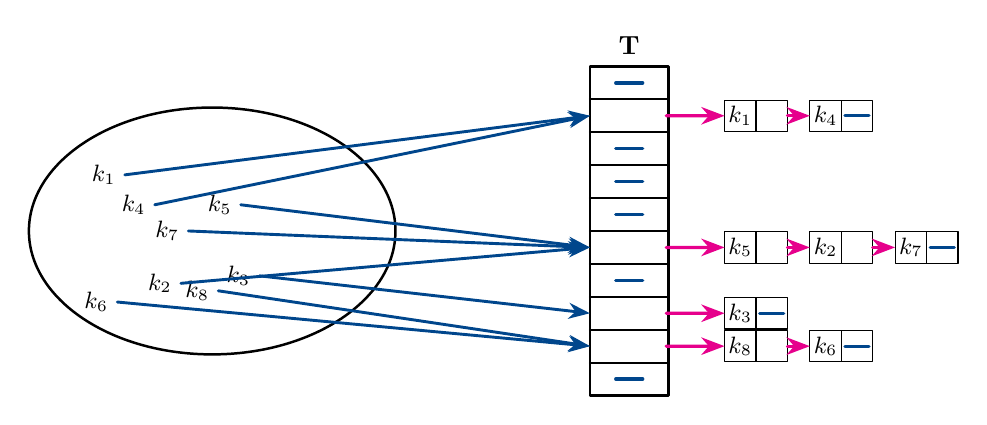
\begin{tikzpicture}[
		x=1cm,y=1cm,
		>=Stealth,
		line cap=round,line join=round,
		font=\small,
		scale=0.95, transform shape
		]
		% ---- colors (gần giống hình)
		\definecolor{hashBlue}{RGB}{0,70,140}
		\definecolor{ptrMagenta}{RGB}{230,0,140}
		
		% ---- parameters
		\def\nrow{10}
		\def\rowH{0.44}
		\def\tw{1.05}
		\def\cell{0.42}
		\def\gap{0.30}
		
		% ---- table position
		\def\xTable{5.05}
		\def\yTable{-2.20} % bottom y
		
		\pgfmathsetmacro{\xTableR}{\xTable+\tw}
		\pgfmathsetmacro{\yTop}{\yTable+\nrow*\rowH}
		
		% row centers (top-based)
		\pgfmathsetmacro{\yRtwo}{\yTop-(2-0.5)*\rowH}
		\pgfmathsetmacro{\yRsix}{\yTop-(6-0.5)*\rowH}
		\pgfmathsetmacro{\yReight}{\yTop-(8-0.5)*\rowH}
		\pgfmathsetmacro{\yRnine}{\yTop-(9-0.5)*\rowH}
		
		% ---- draw table outer + separators
		\coordinate (TBL) at (\xTable,\yTable);
		\coordinate (TTR) at (\xTableR,\yTop);
		\draw[black, line width=0.8pt] (TBL) rectangle (TTR);
		\foreach \i in {1,...,9}{
			\draw[black, line width=0.8pt]
			(\xTable, \yTable+\i*\rowH) -- (\xTableR, \yTable+\i*\rowH);
		}
		\node[font=\bfseries] at ({(\xTable+\xTableR)/2}, {\yTop+0.28}) {T};
		
		% ---- blue dashes inside empty buckets (rows: 1,3,4,5,7,10)
		\foreach \r in {1,3,4,5,7,10}{
			\pgfmathsetmacro{\yc}{\yTop-(\r-0.5)*\rowH}
			\draw[hashBlue, line width=1.2pt]
			({\xTable+\tw/2-0.18},\yc) -- ({\xTable+\tw/2+0.18},\yc);
		}
		
		% ---- ellipse with keys
		\draw[black, line width=0.9pt] (0,0) ellipse (2.45 and 1.65);
		
		\node (K1) at (-1.45, 0.75) {$k_1$};
		\node (K4) at (-1.05, 0.35) {$k_4$};
		\node (K5) at ( 0.10, 0.35) {$k_5$};
		\node (K7) at (-0.60, 0.00) {$k_7$};
		
		\node (K2) at (-0.70,-0.70) {$k_2$};
		\node (K6) at (-1.55,-0.95) {$k_6$};
		\node (K8) at (-0.20,-0.80) {$k_8$};
		\node (K3) at ( 0.35,-0.60) {$k_3$};
		
		% ---- blue hash arrows to table buckets
		\draw[hashBlue, ->, line width=1.05pt] (K1.east) -- (\xTable, \yRtwo);
		\draw[hashBlue, ->, line width=1.05pt] (K4.east) -- (\xTable, \yRtwo);
		
		\draw[hashBlue, ->, line width=1.05pt] (K5.east) -- (\xTable, \yRsix);
		\draw[hashBlue, ->, line width=1.05pt] (K7.east) -- (\xTable, \yRsix);
		\draw[hashBlue, ->, line width=1.05pt] (K2.east) -- (\xTable, \yRsix);
		
		\draw[hashBlue, ->, line width=1.05pt] (K3.east) -- (\xTable, \yReight);
		
		\draw[hashBlue, ->, line width=1.05pt] (K8.east) -- (\xTable, \yRnine);
		\draw[hashBlue, ->, line width=1.05pt] (K6.east) -- (\xTable, \yRnine);
		
		% ===== helper: draw 1 cell (data / next) =====
		% (dùng node vuông, dễ căn)
		\tikzset{
			llcell/.style={draw, minimum width=\cell cm, minimum height=\cell cm, inner sep=0pt, outer sep=0pt}
		}
		
		% ---- Lists start x
		\pgfmathsetmacro{\xList}{\xTableR+0.75}
		
		% ===================== LIST 1: k1 -> k4 -> nil  (row 2) =====================
		\node[llcell] (L1k1) at ({\xList+0.5*\cell}, \yRtwo) {$k_1$};
		\node[llcell] (L1p1) at ({\xList+1.5*\cell}, \yRtwo) {};
		\node[llcell] (L1k4) at ({\xList+2.5*\cell+\gap}, \yRtwo) {$k_4$};
		\node[llcell] (L1p4) at ({\xList+3.5*\cell+\gap}, \yRtwo) {};
		% null mark
		\draw[hashBlue, line width=1.2pt] ($(L1p4.center)+(-0.16,0)$) -- ($(L1p4.center)+(0.16,0)$);
		
		% pointers (magenta)
		\draw[ptrMagenta, ->, line width=1.2pt] ({\xTableR-0.03},\yRtwo) -- (L1k1.west);
		\draw[ptrMagenta, ->, line width=1.2pt] (L1p1.east) -- (L1k4.west);
		
		% ===================== LIST 2: k5 -> k2 -> k7 -> nil (row 6) =====================
		\node[llcell] (L2k5) at ({\xList+0.5*\cell}, \yRsix) {$k_5$};
		\node[llcell] (L2p5) at ({\xList+1.5*\cell}, \yRsix) {};
		\node[llcell] (L2k2) at ({\xList+2.5*\cell+\gap}, \yRsix) {$k_2$};
		\node[llcell] (L2p2) at ({\xList+3.5*\cell+\gap}, \yRsix) {};
		\node[llcell] (L2k7) at ({\xList+4.5*\cell+2*\gap}, \yRsix) {$k_7$};
		\node[llcell] (L2p7) at ({\xList+5.5*\cell+2*\gap}, \yRsix) {};
		\draw[hashBlue, line width=1.2pt] ($(L2p7.center)+(-0.16,0)$) -- ($(L2p7.center)+(0.16,0)$);
		
		\draw[ptrMagenta, ->, line width=1.2pt] ({\xTableR-0.03},\yRsix) -- (L2k5.west);
		\draw[ptrMagenta, ->, line width=1.2pt] (L2p5.east) -- (L2k2.west);
		\draw[ptrMagenta, ->, line width=1.2pt] (L2p2.east) -- (L2k7.west);
		
		% ===================== LIST 3: k3 -> nil (row 8) =====================
		\node[llcell] (L3k3) at ({\xList+0.5*\cell}, \yReight) {$k_3$};
		\node[llcell] (L3p3) at ({\xList+1.5*\cell}, \yReight) {};
		\draw[hashBlue, line width=1.2pt] ($(L3p3.center)+(-0.16,0)$) -- ($(L3p3.center)+(0.16,0)$);
		\draw[ptrMagenta, ->, line width=1.2pt] ({\xTableR-0.03},\yReight) -- (L3k3.west);
		
		% ===================== LIST 4: k8 -> k6 -> nil (row 9) =====================
		\node[llcell] (L4k8) at ({\xList+0.5*\cell}, \yRnine) {$k_8$};
		\node[llcell] (L4p8) at ({\xList+1.5*\cell}, \yRnine) {};
		\node[llcell] (L4k6) at ({\xList+2.5*\cell+\gap}, \yRnine) {$k_6$};
		\node[llcell] (L4p6) at ({\xList+3.5*\cell+\gap}, \yRnine) {};
		\draw[hashBlue, line width=1.2pt] ($(L4p6.center)+(-0.16,0)$) -- ($(L4p6.center)+(0.16,0)$);
		
		\draw[ptrMagenta, ->, line width=1.2pt] ({\xTableR-0.03},\yRnine) -- (L4k8.west);
		\draw[ptrMagenta, ->, line width=1.2pt] (L4p8.east) -- (L4k6.west);
		
	\end{tikzpicture}
\end{frame}

\begin{frame}[t]{2. XUNG ĐỘT VÀ GIẢI QUYẾT XUNG ĐỘT}
	\small
	\setlength{\leftmargini}{-1.2em}
	
	\begin{itemize}
		\item \textbf{Ví dụ:} Giải quyết xung đột theo phương pháp tạo chuỗi
		\begin{itemize}
			\item Một bảng băm được cấp phát $p$ vị trí đánh chỉ số $0, 1, \ldots, p-1$ để lưu trữ cặp khoá - giá trị.
			Bảng băm áp dụng cơ chế tạo chuỗi với hàm dò
			\[
			h(k)=k \ \textit{mod}\ p
			\]
			
			\item Ban đầu, bảng trống rỗng. Hãy vẽ trạng thái bảng (mỗi vị trí chỉ cần ghi khoá nếu đang dùng và ghi ``/'' nếu chưa dùng)
			khi chèn lần lượt các khoá \textbf{22, 1, 13, 11, 24, 33, 18, 42, 31}
			vào bảng với trường hợp $p = 11$.
		\end{itemize}
	\end{itemize}
\end{frame}

% --- SLIDE: Chaining (h(k)=k mod 11) + bảng 0..10 rỗng
\begin{frame}[t]{2. XUNG ĐỘT VÀ GIẢI QUYẾT XUNG ĐỘT}
	\setlength{\leftmargini}{-1.2em}
	
	\begin{columns}[T,onlytextwidth]
		% ---- LEFT: text
		\begin{column}{0.40\textwidth}
			\vspace{0.65cm}
			{\LARGE Chaining}
			
			\vspace{1.25cm}
			{\LARGE $h(k)=k \bmod 11$}
		\end{column}
		
		% ---- RIGHT: sequence + table
		\begin{column}{0.60\textwidth}
			\centering
			{\Large 22, 1, 13, 11, 24, 33, 18, 42, 31}
			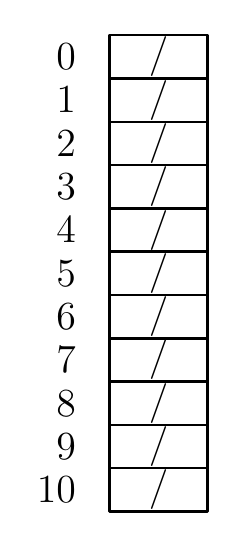
\begin{tikzpicture}[
				x=1cm,y=1cm,
				line cap=round,line join=round
				]
				% ---- parameters
				\def\n{11}          % số hàng
				\def\rowH{0.55}     % chiều cao mỗi ô (cm theo hệ toạ độ tikz)
				\def\tw{1.25}       % chiều rộng bảng (1 cột)
				\def\idxGap{0.30}   % khoảng cách số index tới bảng
				
				% top-left of table
				\coordinate (TL) at (0,0);
				\coordinate (BR) at (\tw, {-\n*\rowH});
				
				% outer border
				\draw[black, line width=0.9pt] (TL) rectangle (BR);
				
				% row separators
				\foreach \i in {1,...,10}{
					\draw[black, line width=0.9pt]
					(0, {-\i*\rowH}) -- (\tw, {-\i*\rowH});
				}
				
				% indices (0..10) + slash inside each cell
				\foreach \i in {0,...,10}{
					\pgfmathsetmacro{\yc}{-(\i+0.5)*\rowH}
					\node[anchor=east, font=\Large] at (-\idxGap, \yc) {\i};
					\node[font=\Large] at ({0.5*\tw}, \yc) {/};
				}
			\end{tikzpicture}
		\end{column}
	\end{columns}
\end{frame}

% --- SLIDE: Ví dụ chaining (bước 1: xử lý 22), highlight 22 + thêm h(22)=0
\begin{frame}[t]{2. XUNG ĐỘT VÀ GIẢI QUYẾT XUNG ĐỘT}
	\small
	\setlength{\leftmargini}{-1.2em}
	
	\begin{itemize}
		\item \textbf{Ví dụ: giải quyết xung đột theo phương pháp tạo chuỗi}
	\end{itemize}
	
	\vspace{0.15cm}
	
	\begin{columns}[T,onlytextwidth]
		% ---- LEFT: text
		\begin{column}{0.58\textwidth}
			\vspace{0.05cm}
			\centering
			{\Large
				\textcolor{orange!85!black}{22}, 1, 13, 11, 24, 33, 18, 42, 31
			}
			
			\vspace{0.55cm}
			{\LARGE Chaining}
			
			\vspace{0.95cm}
			{\Large $h(k)=k \; mod \; 11$}
			
			\vspace{0.25cm}
			{\Large $h(22)=0$}
		\end{column}
		
		% ---- RIGHT: table 0..10 with /
		\begin{column}{0.42\textwidth}
			\centering
			\vspace{-0.05cm}
			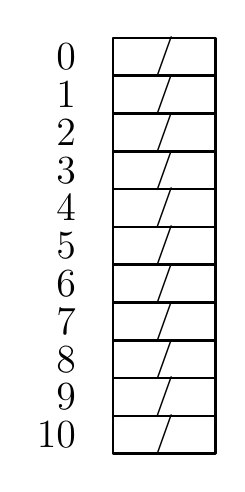
\begin{tikzpicture}[
				x=1cm,y=1cm,
				line cap=round,line join=round
				]
				% ---- parameters
				\def\n{11}
				\def\rowH{0.48}
				\def\tw{1.30}
				\def\idxGap{0.35}
				
				% table corners
				\coordinate (TL) at (0,0);
				\coordinate (BR) at (\tw, {-\n*\rowH});
				
				% outer
				\draw[black, line width=0.9pt] (TL) rectangle (BR);
				
				% separators
				\foreach \i in {1,...,10}{
					\draw[black, line width=0.9pt]
					(0, {-\i*\rowH}) -- (\tw, {-\i*\rowH});
				}
				
				% content
				\foreach \i in {0,...,10}{
					\pgfmathsetmacro{\yc}{-(\i+0.5)*\rowH}
					\node[anchor=east, font=\Large] at (-\idxGap, \yc) {\i};
					\node[font=\Large] at ({0.5*\tw}, \yc) {/};
				}
			\end{tikzpicture}
		\end{column}
	\end{columns}
\end{frame}

% --- SLIDE: bước 1 chèn 22 vào bucket 0 (chaining) - bảng nằm giữa hơn
% --- SLIDE: bước 1 chèn 22 vào bucket 0 (chaining) - DỊCH CỤM BẢNG RA GIỮA BẰNG \hspace*
\begin{frame}[t]{2. XUNG ĐỘT VÀ GIẢI QUYẾT XUNG ĐỘT}
	\small
	\setlength{\leftmargini}{-1.2em}
	
	\begin{itemize}
		\item \textbf{Ví dụ: giải quyết xung đột theo phương pháp tạo chuỗi}
	\end{itemize}
	
	\vspace{0.05cm}
	\centering
	{\Large \textcolor{orange!85!black}{22}, 1, 13, 11, 24, 33, 18, 42, 31}
	
	\vspace{0.15cm}
	
	\begin{columns}[T,onlytextwidth]
		% ---- LEFT (hẹp để chừa chỗ cho hình bên phải về sau)
		\begin{column}{0.34\textwidth}
			\vspace{0.15cm}
			\centering
			{\LARGE Chaining}
			
			\vspace{0.95cm}
			{\Large $h(k)=k \ \mathrm{mod}\ 11$}
			
			\vspace{0.25cm}
			{\Large $h(22)=0$}
		\end{column}
		
		% ---- RIGHT (rộng để về sau vẽ chain dài)
		\begin{column}{0.66\textwidth}
			\vspace{-0.10cm}
			
			% ====== DỊCH CẢ CỤM (BẢNG + LIST) SANG TRÁI: âm nhiều hơn -> ra giữa hơn
			\hspace*{-1.20cm} % bạn có thể thử -0.8 / -1.0 / -1.4 tuỳ slide
			
			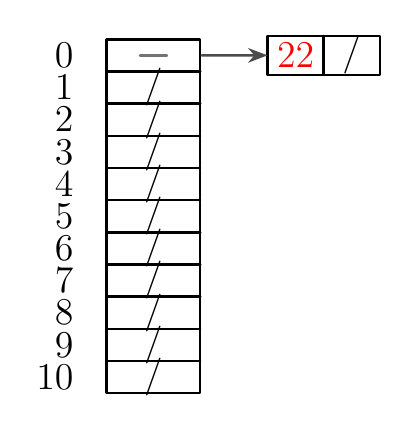
\begin{tikzpicture}[x=1cm,y=1cm, line cap=round,line join=round,>=Stealth,
				scale=0.95, transform shape]
				
				% ---- parameters (đủ gọn để không thừa xuống dưới)
				\def\nRows{11}
				\def\rowH{0.43}
				\def\tw{1.25}
				\def\idxGap{0.32}
				
				% table corners
				\coordinate (TL) at (0,0);
				\coordinate (BR) at (\tw, {-\nRows*\rowH});
				
				% outer + separators
				\draw[black, line width=0.9pt] (TL) rectangle (BR);
				\foreach \i in {1,...,10}{
					\draw[black, line width=0.9pt] (0, {-\i*\rowH}) -- (\tw, {-\i*\rowH});
				}
				
				% indices + content
				\foreach \i in {0,...,10}{
					\pgfmathsetmacro{\yCenter}{-(\i+0.5)*\rowH}
					\node[anchor=east, font=\Large] at (-\idxGap, \yCenter) {\i};
					
					\ifnum\i=0
					% row 0: dấu gạch nhỏ (ô đang trỏ ra ngoài)
					\draw[black!55, line width=0.9pt]
					({0.5*\tw-0.18},\yCenter) -- ({0.5*\tw+0.18},\yCenter);
					\else
					\node[font=\Large] at ({0.5*\tw}, \yCenter) {/};
					\fi
				}
				
				% ---- anchor at row 0 (right edge of table)
				\coordinate (Pzero) at (\tw, {-(0.5)*\rowH});
				
				% ---- node [22 | /]
				\def\cellW{0.75}
				\def\cellH{0.52}
				\def\halfH{0.26} % cellH/2
				
				% bottom-left of node block (đặt ngay bên phải bucket 0)
				\coordinate (NBL) at ($(Pzero)+(0.90,-\halfH)$);
				
				% draw 2-cell block
				\draw[black, line width=0.9pt] (NBL) rectangle ++(\cellW,\cellH);
				\draw[black, line width=0.9pt] ($(NBL)+(\cellW,0)$) rectangle ++(\cellW,\cellH);
				\draw[black, line width=0.9pt] ($(NBL)+(\cellW,0)$) -- ($(NBL)+(\cellW,\cellH)$);
				
				\node[font=\Large, text=red] at ($(NBL)+(0.5*\cellW,0.5*\cellH)$) {22};
				\node[font=\Large]          at ($(NBL)+(1.5*\cellW,0.5*\cellH)$) {/};
				
				% arrow from bucket 0 -> node
				\draw[->, black!70, line width=0.9pt]
				($(Pzero)+(0.02,0)$) -- ($(NBL)+(0,0.5*\cellH)$);
				
			\end{tikzpicture}
		\end{column}
	\end{columns}
\end{frame}

% =========================
% (19) Xử lý phần tử 1 (chưa chèn vào bảng)  --- NODE ĐÃ THU NHỎ
% =========================
\begin{frame}[t]{2. XUNG ĐỘT VÀ GIẢI QUYẾT XUNG ĐỘT}
	\small
	\setlength{\leftmargini}{-1.2em}
	\definecolor{hashBlue}{RGB}{0,70,140}
	
	\begin{itemize}
		\item \textbf{Ví dụ: giải quyết xung đột theo phương pháp tạo chuỗi}
	\end{itemize}
	
	\vspace{0.05cm}
	\centering
	{\Large \textcolor{hashBlue}{22}, \textcolor{red}{1}, 13, 11, 24, 33, 18, 42, 31}
	
	\vspace{0.15cm}
	
	\begin{columns}[T,onlytextwidth]
		\begin{column}{0.34\textwidth}
			\vspace{0.15cm}
			\centering
			{\LARGE Chaining}
			
			\vspace{0.95cm}
			{\Large $h(k)=k \; mod \; 11$}
			
			\vspace{0.25cm}
			{\Large $h(1)=1$}
		\end{column}
		
		\begin{column}{0.66\textwidth}
			\vspace{-0.10cm}
			\hspace*{-1.20cm}
			
			\begin{tikzpicture}[x=1cm,y=1cm, line cap=round,line join=round,>=Stealth,
				scale=0.95, transform shape]
				
				% ---- table parameters
				\def\nRows{11}
				\def\rowH{0.43}
				\def\tw{1.25}
				\def\idxGap{0.32}
				
				% ---- node parameters (ĐÃ THU NHỎ để không đè nhau)
				\def\cellW{0.70}
				\def\cellH{0.36}
				\def\halfH{0.18}
				
				\coordinate (TL) at (0,0);
				\coordinate (BR) at (\tw, {-\nRows*\rowH});
				
				\draw[black, line width=0.9pt] (TL) rectangle (BR);
				\foreach \i in {1,...,10}{
					\draw[black, line width=0.9pt] (0, {-\i*\rowH}) -- (\tw, {-\i*\rowH});
				}
				
				% indices + content (row 0: dash, others: /)
				\foreach \i in {0,...,10}{
					\pgfmathsetmacro{\yC}{-(\i+0.5)*\rowH}
					\node[anchor=east, font=\Large] at (-\idxGap, \yC) {\i};
					
					\ifnum\i=0
					\draw[black!55, line width=0.9pt] ({0.5*\tw-0.18},\yC) -- ({0.5*\tw+0.18},\yC);
					\else
					\node[font=\Large] at ({0.5*\tw}, \yC) {/};
					\fi
				}
				
				% -------- bucket 0 -> node 22
				\coordinate (P0) at (\tw, {-(0.5)*\rowH});
				\coordinate (N0) at ($(P0)+(0.90,-\halfH)$);
				
				\draw[black, line width=0.9pt] (N0) rectangle ++(\cellW,\cellH);
				\draw[black, line width=0.9pt] ($(N0)+(\cellW,0)$) rectangle ++(\cellW,\cellH);
				\draw[black, line width=0.9pt] ($(N0)+(\cellW,0)$) -- ($(N0)+(\cellW,\cellH)$);
				
				\node[font=\normalsize, text=red] at ($(N0)+(0.5*\cellW,0.5*\cellH)$) {22};
				\draw[hashBlue, line width=0.9pt]
				($(N0)+(1.5*\cellW,0.5*\cellH)+(-0.08,-0.14)$) --
				($(N0)+(1.5*\cellW,0.5*\cellH)+( 0.08, 0.14)$);
				
				\draw[->, black!70, line width=0.9pt] ($(P0)+(0.02,0)$) -- ($(N0)+(0,0.5*\cellH)$);
			\end{tikzpicture}
		\end{column}
	\end{columns}
\end{frame}


% =========================
% (20) Chèn 1 vào bucket 1  --- NODE ĐÃ THU NHỎ
% =========================
\begin{frame}[t]{2. XUNG ĐỘT VÀ GIẢI QUYẾT XUNG ĐỘT}
	\small
	\setlength{\leftmargini}{-1.2em}
	\definecolor{hashBlue}{RGB}{0,70,140}
	
	\begin{itemize}
		\item \textbf{Ví dụ: giải quyết xung đột theo phương pháp tạo chuỗi}
	\end{itemize}
	
	\vspace{0.05cm}
	\centering
	{\Large \textcolor{hashBlue}{22}, \textcolor{red}{1}, 13, 11, 24, 33, 18, 42, 31}
	
	\vspace{0.15cm}
	
	\begin{columns}[T,onlytextwidth]
		\begin{column}{0.34\textwidth}
			\vspace{0.15cm}
			\centering
			{\LARGE Chaining}
			
			\vspace{0.95cm}
			{\Large $h(k)=k \; mod \; 11$}
			
			\vspace{0.25cm}
			{\Large $h(1)=1$}
		\end{column}
		
		\begin{column}{0.66\textwidth}
			\vspace{-0.10cm}
			\hspace*{-1.20cm}
			
			\begin{tikzpicture}[x=1cm,y=1cm, line cap=round,line join=round,>=Stealth,
				scale=0.95, transform shape]
				
				\def\nRows{11}
				\def\rowH{0.43}
				\def\tw{1.25}
				\def\idxGap{0.32}
				
				% node nhỏ để không đè nhau
				\def\cellW{0.70}
				\def\cellH{0.36}
				\def\halfH{0.18}
				
				\coordinate (TL) at (0,0);
				\coordinate (BR) at (\tw, {-\nRows*\rowH});
				
				\draw[black, line width=0.9pt] (TL) rectangle (BR);
				\foreach \i in {1,...,10}{
					\draw[black, line width=0.9pt] (0, {-\i*\rowH}) -- (\tw, {-\i*\rowH});
				}
				
				% indices + content (rows 0,1: dash; others: /)
				\foreach \i in {0,...,10}{
					\pgfmathsetmacro{\yC}{-(\i+0.5)*\rowH}
					\node[anchor=east, font=\Large] at (-\idxGap, \yC) {\i};
					
					\ifnum\i=0
					\draw[black!55, line width=0.9pt] ({0.5*\tw-0.18},\yC) -- ({0.5*\tw+0.18},\yC);
					\else\ifnum\i=1
					\draw[black!55, line width=0.9pt] ({0.5*\tw-0.18},\yC) -- ({0.5*\tw+0.18},\yC);
					\else
					\draw[black, line width=0.9pt]
					({0.5*\tw-0.10}, {\yC-0.16}) -- ({0.5*\tw+0.10}, {\yC+0.16});
					\fi\fi
				}
				
				% bucket 0 -> 22
				\coordinate (P0) at (\tw, {-(0.5)*\rowH});
				\coordinate (N0) at ($(P0)+(0.90,-\halfH)$);
				\draw[black, line width=0.9pt] (N0) rectangle ++(\cellW,\cellH);
				\draw[black, line width=0.9pt] ($(N0)+(\cellW,0)$) rectangle ++(\cellW,\cellH);
				\draw[black, line width=0.9pt] ($(N0)+(\cellW,0)$) -- ($(N0)+(\cellW,\cellH)$);
				\node[font=\normalsize, text=red] at ($(N0)+(0.5*\cellW,0.5*\cellH)$) {22};
				\draw[hashBlue, line width=0.9pt]
				($(N0)+(1.5*\cellW,0.5*\cellH)+(-0.08,-0.14)$) --
				($(N0)+(1.5*\cellW,0.5*\cellH)+( 0.08, 0.14)$);
				\draw[->, black!70, line width=0.9pt] ($(P0)+(0.02,0)$) -- ($(N0)+(0,0.5*\cellH)$);
				
				% bucket 1 -> 1
				\coordinate (P1) at (\tw, {-(1.5)*\rowH});
				\coordinate (N1) at ($(P1)+(0.90,-\halfH)$);
				\draw[black, line width=0.9pt] (N1) rectangle ++(\cellW,\cellH);
				\draw[black, line width=0.9pt] ($(N1)+(\cellW,0)$) rectangle ++(\cellW,\cellH);
				\draw[black, line width=0.9pt] ($(N1)+(\cellW,0)$) -- ($(N1)+(\cellW,\cellH)$);
				\node[font=\normalsize, text=red] at ($(N1)+(0.5*\cellW,0.5*\cellH)$) {1};
				\draw[hashBlue, line width=0.9pt]
				($(N1)+(1.5*\cellW,0.5*\cellH)+(-0.08,-0.14)$) --
				($(N1)+(1.5*\cellW,0.5*\cellH)+( 0.08, 0.14)$);
				\draw[->, black!70, line width=0.9pt] ($(P1)+(0.02,0)$) -- ($(N1)+(0,0.5*\cellH)$);
				
			\end{tikzpicture}
		\end{column}
	\end{columns}
\end{frame}


% =========================
% (21) Xử lý phần tử 13 (chưa chèn)  --- NODE ĐÃ THU NHỎ
% =========================
\begin{frame}[t]{2. XUNG ĐỘT VÀ GIẢI QUYẾT XUNG ĐỘT}
	\small
	\setlength{\leftmargini}{-1.2em}
	\definecolor{hashBlue}{RGB}{0,70,140}
	
	\begin{itemize}
		\item \textbf{Ví dụ: giải quyết xung đột theo phương pháp tạo chuỗi}
	\end{itemize}
	
	\vspace{0.05cm}
	\centering
	{\Large \textcolor{hashBlue}{22}, \textcolor{hashBlue}{1}, \textcolor{orange!85!black}{13}, 11, 24, 33, 18, 42, 31}
	
	\vspace{0.15cm}
	
	\begin{columns}[T,onlytextwidth]
		\begin{column}{0.34\textwidth}
			\vspace{0.15cm}
			\centering
			{\LARGE Chaining}
			
			\vspace{0.95cm}
			{\Large $h(k)=k \; mod \; 11$}
			
			\vspace{0.25cm}
			{\Large $h(13)=2$}
		\end{column}
		
		\begin{column}{0.66\textwidth}
			\vspace{-0.10cm}
			\hspace*{-1.20cm}
			
			\begin{tikzpicture}[x=1cm,y=1cm, line cap=round,line join=round,>=Stealth,
				scale=0.95, transform shape]
				
				\def\nRows{11}
				\def\rowH{0.43}
				\def\tw{1.25}
				\def\idxGap{0.32}
				
				% node nhỏ để không đè
				\def\cellW{0.70}
				\def\cellH{0.36}
				\def\halfH{0.18}
				
				\coordinate (TL) at (0,0);
				\coordinate (BR) at (\tw, {-\nRows*\rowH});
				
				\draw[black, line width=0.9pt] (TL) rectangle (BR);
				\foreach \i in {1,...,10}{
					\draw[black, line width=0.9pt] (0, {-\i*\rowH}) -- (\tw, {-\i*\rowH});
				}
				
				% rows 0,1: dash; others: /
				\foreach \i in {0,...,10}{
					\pgfmathsetmacro{\yC}{-(\i+0.5)*\rowH}
					\node[anchor=east, font=\Large] at (-\idxGap, \yC) {\i};
					
					\ifnum\i=0
					\draw[black!55, line width=0.9pt] ({0.5*\tw-0.18},\yC) -- ({0.5*\tw+0.18},\yC);
					\else\ifnum\i=1
					\draw[black!55, line width=0.9pt] ({0.5*\tw-0.18},\yC) -- ({0.5*\tw+0.18},\yC);
					\else
					\draw[black, line width=0.9pt]
					({0.5*\tw-0.10}, {\yC-0.16}) -- ({0.5*\tw+0.10}, {\yC+0.16});
					\fi\fi
				}
				
				% bucket 0 -> 22
				\coordinate (P0) at (\tw, {-(0.5)*\rowH});
				\coordinate (N0) at ($(P0)+(0.90,-\halfH)$);
				\draw[black, line width=0.9pt] (N0) rectangle ++(\cellW,\cellH);
				\draw[black, line width=0.9pt] ($(N0)+(\cellW,0)$) rectangle ++(\cellW,\cellH);
				\draw[black, line width=0.9pt] ($(N0)+(\cellW,0)$) -- ($(N0)+(\cellW,\cellH)$);
				\node[font=\normalsize, text=red] at ($(N0)+(0.5*\cellW,0.5*\cellH)$) {22};
				\draw[hashBlue, line width=0.9pt]
				($(N0)+(1.5*\cellW,0.5*\cellH)+(-0.08,-0.14)$) --
				($(N0)+(1.5*\cellW,0.5*\cellH)+( 0.08, 0.14)$);
				\draw[->, black!70, line width=0.9pt] ($(P0)+(0.02,0)$) -- ($(N0)+(0,0.5*\cellH)$);
				
				% bucket 1 -> 1
				\coordinate (P1) at (\tw, {-(1.5)*\rowH});
				\coordinate (N1) at ($(P1)+(0.90,-\halfH)$);
				\draw[black, line width=0.9pt] (N1) rectangle ++(\cellW,\cellH);
				\draw[black, line width=0.9pt] ($(N1)+(\cellW,0)$) rectangle ++(\cellW,\cellH);
				\draw[black, line width=0.9pt] ($(N1)+(\cellW,0)$) -- ($(N1)+(\cellW,\cellH)$);
				\node[font=\normalsize, text=red] at ($(N1)+(0.5*\cellW,0.5*\cellH)$) {1};
				\draw[hashBlue, line width=0.9pt]
				($(N1)+(1.5*\cellW,0.5*\cellH)+(-0.08,-0.14)$) --
				($(N1)+(1.5*\cellW,0.5*\cellH)+( 0.08, 0.14)$);
				\draw[->, black!70, line width=0.9pt] ($(P1)+(0.02,0)$) -- ($(N1)+(0,0.5*\cellH)$);
				
			\end{tikzpicture}
		\end{column}
	\end{columns}
\end{frame}


% =========================
% (22) Chèn 13 vào bucket 2  --- NODE ĐÃ THU NHỎ
% =========================
\begin{frame}[t]{2. XUNG ĐỘT VÀ GIẢI QUYẾT XUNG ĐỘT}
	\small
	\setlength{\leftmargini}{-1.2em}
	\definecolor{hashBlue}{RGB}{0,70,140}
	
	\begin{itemize}
		\item \textbf{Ví dụ: giải quyết xung đột theo phương pháp tạo chuỗi}
	\end{itemize}
	
	\vspace{0.05cm}
	\centering
	{\Large \textcolor{hashBlue}{22}, \textcolor{hashBlue}{1}, \textcolor{orange!85!black}{13}, 11, 24, 33, 18, 42, 31}
	
	\vspace{0.15cm}
	
	\begin{columns}[T,onlytextwidth]
		\begin{column}{0.34\textwidth}
			\vspace{0.15cm}
			\centering
			{\LARGE Chaining}
			
			\vspace{0.95cm}
			{\Large $h(k)=k \; mod \; 11$}
			
			\vspace{0.25cm}
			{\Large $h(13)=2$}
		\end{column}
		
		\begin{column}{0.66\textwidth}
			\vspace{-0.10cm}
			\hspace*{-1.20cm}
			
			\begin{tikzpicture}[x=1cm,y=1cm, line cap=round,line join=round,>=Stealth,
				scale=0.95, transform shape]
				
				\def\nRows{11}
				\def\rowH{0.43}
				\def\tw{1.25}
				\def\idxGap{0.32}
				
				% node nhỏ
				\def\cellW{0.70}
				\def\cellH{0.36}
				\def\halfH{0.18}
				
				\coordinate (TL) at (0,0);
				\coordinate (BR) at (\tw, {-\nRows*\rowH});
				
				\draw[black, line width=0.9pt] (TL) rectangle (BR);
				\foreach \i in {1,...,10}{
					\draw[black, line width=0.9pt] (0, {-\i*\rowH}) -- (\tw, {-\i*\rowH});
				}
				
				% rows 0,1,2: dash; others: /
				\foreach \i in {0,...,10}{
					\pgfmathsetmacro{\yC}{-(\i+0.5)*\rowH}
					\node[anchor=east, font=\Large] at (-\idxGap, \yC) {\i};
					
					\ifnum\i=0
					\draw[black!55, line width=0.9pt] ({0.5*\tw-0.18},\yC) -- ({0.5*\tw+0.18},\yC);
					\else\ifnum\i=1
					\draw[black!55, line width=0.9pt] ({0.5*\tw-0.18},\yC) -- ({0.5*\tw+0.18},\yC);
					\else\ifnum\i=2
					\draw[black!55, line width=0.9pt] ({0.5*\tw-0.18},\yC) -- ({0.5*\tw+0.18},\yC);
					\else
					\draw[black, line width=0.9pt]
					({0.5*\tw-0.10}, {\yC-0.16}) -- ({0.5*\tw+0.10}, {\yC+0.16});
					\fi\fi\fi
				}
				
				% bucket 0 -> 22
				\coordinate (P0) at (\tw, {-(0.5)*\rowH});
				\coordinate (N0) at ($(P0)+(0.90,-\halfH)$);
				\draw[black, line width=0.9pt] (N0) rectangle ++(\cellW,\cellH);
				\draw[black, line width=0.9pt] ($(N0)+(\cellW,0)$) rectangle ++(\cellW,\cellH);
				\draw[black, line width=0.9pt] ($(N0)+(\cellW,0)$) -- ($(N0)+(\cellW,\cellH)$);
				\node[font=\normalsize, text=red] at ($(N0)+(0.5*\cellW,0.5*\cellH)$) {22};
				\draw[hashBlue, line width=0.9pt]
				($(N0)+(1.5*\cellW,0.5*\cellH)+(-0.08,-0.14)$) --
				($(N0)+(1.5*\cellW,0.5*\cellH)+( 0.08, 0.14)$);
				\draw[->, black!70, line width=0.9pt] ($(P0)+(0.02,0)$) -- ($(N0)+(0,0.5*\cellH)$);
				
				% bucket 1 -> 1
				\coordinate (P1) at (\tw, {-(1.5)*\rowH});
				\coordinate (N1) at ($(P1)+(0.90,-\halfH)$);
				\draw[black, line width=0.9pt] (N1) rectangle ++(\cellW,\cellH);
				\draw[black, line width=0.9pt] ($(N1)+(\cellW,0)$) rectangle ++(\cellW,\cellH);
				\draw[black, line width=0.9pt] ($(N1)+(\cellW,0)$) -- ($(N1)+(\cellW,\cellH)$);
				\node[font=\normalsize, text=red] at ($(N1)+(0.5*\cellW,0.5*\cellH)$) {1};
				\draw[hashBlue, line width=0.9pt]
				($(N1)+(1.5*\cellW,0.5*\cellH)+(-0.08,-0.14)$) --
				($(N1)+(1.5*\cellW,0.5*\cellH)+( 0.08, 0.14)$);
				\draw[->, black!70, line width=0.9pt] ($(P1)+(0.02,0)$) -- ($(N1)+(0,0.5*\cellH)$);
				
				% bucket 2 -> 13
				\coordinate (P2) at (\tw, {-(2.5)*\rowH});
				\coordinate (N2) at ($(P2)+(0.90,-\halfH)$);
				\draw[black, line width=0.9pt] (N2) rectangle ++(\cellW,\cellH);
				\draw[black, line width=0.9pt] ($(N2)+(\cellW,0)$) rectangle ++(\cellW,\cellH);
				\draw[black, line width=0.9pt] ($(N2)+(\cellW,0)$) -- ($(N2)+(\cellW,\cellH)$);
				\node[font=\normalsize, text=red] at ($(N2)+(0.5*\cellW,0.5*\cellH)$) {13};
				\draw[hashBlue, line width=0.9pt]
				($(N2)+(1.5*\cellW,0.5*\cellH)+(-0.08,-0.14)$) --
				($(N2)+(1.5*\cellW,0.5*\cellH)+( 0.08, 0.14)$);
				\draw[->, black!70, line width=0.9pt] ($(P2)+(0.02,0)$) -- ($(N2)+(0,0.5*\cellH)$);
				
			\end{tikzpicture}
		\end{column}
	\end{columns}
\end{frame}


% =========================
% (23) Xử lý phần tử 11 (chưa chèn)  --- NODE ĐÃ THU NHỎ
% =========================
\begin{frame}[t]{2. XUNG ĐỘT VÀ GIẢI QUYẾT XUNG ĐỘT}
	\small
	\setlength{\leftmargini}{-1.2em}
	\definecolor{hashBlue}{RGB}{0,70,140}
	
	\begin{itemize}
		\item \textbf{Ví dụ: giải quyết xung đột theo phương pháp tạo chuỗi}
	\end{itemize}
	
	\vspace{0.05cm}
	\centering
	{\Large \textcolor{hashBlue}{22}, \textcolor{hashBlue}{1}, \textcolor{hashBlue}{13}, \textcolor{red}{11}, 24, 33, 18, 42, 31}
	
	\vspace{0.15cm}
	
	\begin{columns}[T,onlytextwidth]
		\begin{column}{0.34\textwidth}
			\vspace{0.15cm}
			\centering
			{\LARGE Chaining}
			
			\vspace{0.95cm}
			{\Large $h(k)=k \; mod \; 11$}
			
			\vspace{0.25cm}
			{\Large $h(11)=0$}
		\end{column}
		
		\begin{column}{0.66\textwidth}
			\vspace{-0.10cm}
			\hspace*{-1.20cm}
			
			\begin{tikzpicture}[x=1cm,y=1cm, line cap=round,line join=round,>=Stealth,
				scale=0.95, transform shape]
				
				\def\nRows{11}
				\def\rowH{0.43}
				\def\tw{1.25}
				\def\idxGap{0.32}
				
				% node nhỏ
				\def\cellW{0.70}
				\def\cellH{0.36}
				\def\halfH{0.18}
				
				\coordinate (TL) at (0,0);
				\coordinate (BR) at (\tw, {-\nRows*\rowH});
				
				\draw[black, line width=0.9pt] (TL) rectangle (BR);
				\foreach \i in {1,...,10}{
					\draw[black, line width=0.9pt] (0, {-\i*\rowH}) -- (\tw, {-\i*\rowH});
				}
				
				% rows 0,1,2: dash; others: /
				\foreach \i in {0,...,10}{
					\pgfmathsetmacro{\yC}{-(\i+0.5)*\rowH}
					\node[anchor=east, font=\Large] at (-\idxGap, \yC) {\i};
					
					\ifnum\i=0
					\draw[black!55, line width=0.9pt] ({0.5*\tw-0.18},\yC) -- ({0.5*\tw+0.18},\yC);
					\else\ifnum\i=1
					\draw[black!55, line width=0.9pt] ({0.5*\tw-0.18},\yC) -- ({0.5*\tw+0.18},\yC);
					\else\ifnum\i=2
					\draw[black!55, line width=0.9pt] ({0.5*\tw-0.18},\yC) -- ({0.5*\tw+0.18},\yC);
					\else
					\draw[black, line width=0.9pt]
					({0.5*\tw-0.10}, {\yC-0.16}) -- ({0.5*\tw+0.10}, {\yC+0.16});
					\fi\fi\fi
				}
				
				% bucket 0 -> 22
				\coordinate (P0) at (\tw, {-(0.5)*\rowH});
				\coordinate (N0) at ($(P0)+(0.90,-\halfH)$);
				\draw[black, line width=0.9pt] (N0) rectangle ++(\cellW,\cellH);
				\draw[black, line width=0.9pt] ($(N0)+(\cellW,0)$) rectangle ++(\cellW,\cellH);
				\draw[black, line width=0.9pt] ($(N0)+(\cellW,0)$) -- ($(N0)+(\cellW,\cellH)$);
				\node[font=\normalsize, text=red] at ($(N0)+(0.5*\cellW,0.5*\cellH)$) {22};
				\draw[hashBlue, line width=0.9pt]
				($(N0)+(1.5*\cellW,0.5*\cellH)+(-0.08,-0.14)$) --
				($(N0)+(1.5*\cellW,0.5*\cellH)+( 0.08, 0.14)$);
				\draw[->, black!70, line width=0.9pt] ($(P0)+(0.02,0)$) -- ($(N0)+(0,0.5*\cellH)$);
				
				% bucket 1 -> 1
				\coordinate (P1) at (\tw, {-(1.5)*\rowH});
				\coordinate (N1) at ($(P1)+(0.90,-\halfH)$);
				\draw[black, line width=0.9pt] (N1) rectangle ++(\cellW,\cellH);
				\draw[black, line width=0.9pt] ($(N1)+(\cellW,0)$) rectangle ++(\cellW,\cellH);
				\draw[black, line width=0.9pt] ($(N1)+(\cellW,0)$) -- ($(N1)+(\cellW,\cellH)$);
				\node[font=\normalsize, text=red] at ($(N1)+(0.5*\cellW,0.5*\cellH)$) {1};
				\draw[hashBlue, line width=0.9pt]
				($(N1)+(1.5*\cellW,0.5*\cellH)+(-0.08,-0.14)$) --
				($(N1)+(1.5*\cellW,0.5*\cellH)+( 0.08, 0.14)$);
				\draw[->, black!70, line width=0.9pt] ($(P1)+(0.02,0)$) -- ($(N1)+(0,0.5*\cellH)$);
				
				% bucket 2 -> 13
				\coordinate (P2) at (\tw, {-(2.5)*\rowH});
				\coordinate (N2) at ($(P2)+(0.90,-\halfH)$);
				\draw[black, line width=0.9pt] (N2) rectangle ++(\cellW,\cellH);
				\draw[black, line width=0.9pt] ($(N2)+(\cellW,0)$) rectangle ++(\cellW,\cellH);
				\draw[black, line width=0.9pt] ($(N2)+(\cellW,0)$) -- ($(N2)+(\cellW,\cellH)$);
				\node[font=\normalsize, text=red] at ($(N2)+(0.5*\cellW,0.5*\cellH)$) {13};
				\draw[hashBlue, line width=0.9pt]
				($(N2)+(1.5*\cellW,0.5*\cellH)+(-0.08,-0.14)$) --
				($(N2)+(1.5*\cellW,0.5*\cellH)+( 0.08, 0.14)$);
				\draw[->, black!70, line width=0.9pt] ($(P2)+(0.02,0)$) -- ($(N2)+(0,0.5*\cellH)$);
				
			\end{tikzpicture}
		\end{column}
	\end{columns}
\end{frame}

% =========================================================
% (24) CHÈN 11 vào bucket 0  -> 11 -> 22
% =========================================================
\begin{frame}[t]{2. XUNG ĐỘT VÀ GIẢI QUYẾT XUNG ĐỘT}
	\small
	\setlength{\leftmargini}{-1.2em}
	\definecolor{hashBlue}{RGB}{0,70,140}
	
	\begin{itemize}
		\item \textbf{Ví dụ: giải quyết xung đột theo phương pháp tạo chuỗi}
	\end{itemize}
	
	\vspace{0.05cm}
	\centering
	{\Large \textcolor{hashBlue}{22}, \textcolor{hashBlue}{1}, \textcolor{hashBlue}{13}, \textcolor{red}{11}, 24, 33, 18, 42, 31}
	
	\vspace{0.15cm}
	
	\begin{columns}[T,onlytextwidth]
		\begin{column}{0.34\textwidth}
			\vspace{0.15cm}
			\centering
			{\LARGE Chaining}
			
			\vspace{0.95cm}
			{\Large $h(k)=k \; mod \; 11$}
			
			\vspace{0.25cm}
			{\Large $h(11)=0$}
		\end{column}
		
		\begin{column}{0.66\textwidth}
			\vspace{-0.10cm}
			\hspace*{-1.20cm}
			
			\begin{tikzpicture}[x=1cm,y=1cm, line cap=round,line join=round,>=Stealth,
				scale=0.95, transform shape]
				
				\def\nRows{11}
				\def\rowH{0.43}
				\def\tw{1.25}
				\def\idxGap{0.32}
				
				% node nhỏ + khoảng cách chain
				\def\cellW{0.70}
				\def\cellH{0.36}
				\def\halfH{0.18}
				\def\gap{0.45}
				
				% table
				\coordinate (TL) at (0,0);
				\coordinate (BR) at (\tw, {-\nRows*\rowH});
				
				\draw[black, line width=0.9pt] (TL) rectangle (BR);
				\foreach \i in {1,...,10}{
					\draw[black, line width=0.9pt] (0, {-\i*\rowH}) -- (\tw, {-\i*\rowH});
				}
				
				% dashes at rows 0,1,2 ; others short slashes
				\foreach \i in {0,...,10}{
					\pgfmathsetmacro{\yC}{-(\i+0.5)*\rowH}
					\node[anchor=east, font=\Large] at (-\idxGap, \yC) {\i};
					
					\ifnum\i=0
					\draw[black!55, line width=0.9pt] ({0.5*\tw-0.18},\yC) -- ({0.5*\tw+0.18},\yC);
					\else\ifnum\i=1
					\draw[black!55, line width=0.9pt] ({0.5*\tw-0.18},\yC) -- ({0.5*\tw+0.18},\yC);
					\else\ifnum\i=2
					\draw[black!55, line width=0.9pt] ({0.5*\tw-0.18},\yC) -- ({0.5*\tw+0.18},\yC);
					\else
					\draw[black, line width=0.9pt]
					({0.5*\tw-0.10}, {\yC-0.16}) -- ({0.5*\tw+0.10}, {\yC+0.16});
					\fi\fi\fi
				}
				
				% ======================
				% bucket 0 : 11 -> 22
				% ======================
				\coordinate (P0) at (\tw, {-(0.5)*\rowH});
				\coordinate (N0a) at ($(P0)+(0.90,-\halfH)$); % 11 (new head)
				\coordinate (N0b) at ($(N0a)+(2*\cellW+\gap,0)$); % 22
				
				% node 11 (right cell blank)
				\draw[black, line width=0.9pt] (N0a) rectangle ++(\cellW,\cellH);
				\draw[black, line width=0.9pt] ($(N0a)+(\cellW,0)$) rectangle ++(\cellW,\cellH);
				\draw[black, line width=0.9pt] ($(N0a)+(\cellW,0)$) -- ($(N0a)+(\cellW,\cellH)$);
				\node[font=\normalsize, text=red] at ($(N0a)+(0.5*\cellW,0.5*\cellH)$) {11};
				
				% node 22 (last => slash)
				\draw[black, line width=0.9pt] (N0b) rectangle ++(\cellW,\cellH);
				\draw[black, line width=0.9pt] ($(N0b)+(\cellW,0)$) rectangle ++(\cellW,\cellH);
				\draw[black, line width=0.9pt] ($(N0b)+(\cellW,0)$) -- ($(N0b)+(\cellW,\cellH)$);
				\node[font=\normalsize, text=black] at ($(N0b)+(0.5*\cellW,0.5*\cellH)$) {22};
				\draw[hashBlue, line width=0.9pt]
				($(N0b)+(1.5*\cellW,0.5*\cellH)+(-0.08,-0.14)$) --
				($(N0b)+(1.5*\cellW,0.5*\cellH)+( 0.08, 0.14)$);
				
				% arrows
				\draw[->, black!70, line width=0.9pt] ($(P0)+(0.02,0)$) -- ($(N0a)+(0,0.5*\cellH)$);
				\draw[->, black!70, line width=0.9pt] ($(N0a)+(2*\cellW,0.5*\cellH)$) -- ($(N0b)+(0,0.5*\cellH)$);
				
				
				% ======================
				% bucket 1 : 1 (last)
				% ======================
				\coordinate (P1) at (\tw, {-(1.5)*\rowH});
				\coordinate (N1) at ($(P1)+(0.90,-\halfH)$);
				\draw[black, line width=0.9pt] (N1) rectangle ++(\cellW,\cellH);
				\draw[black, line width=0.9pt] ($(N1)+(\cellW,0)$) rectangle ++(\cellW,\cellH);
				\draw[black, line width=0.9pt] ($(N1)+(\cellW,0)$) -- ($(N1)+(\cellW,\cellH)$);
				\node[font=\normalsize, text=black] at ($(N1)+(0.5*\cellW,0.5*\cellH)$) {1};
				\draw[hashBlue, line width=0.9pt]
				($(N1)+(1.5*\cellW,0.5*\cellH)+(-0.08,-0.14)$) --
				($(N1)+(1.5*\cellW,0.5*\cellH)+( 0.08, 0.14)$);
				\draw[->, black!70, line width=0.9pt] ($(P1)+(0.02,0)$) -- ($(N1)+(0,0.5*\cellH)$);
				
				
				% ======================
				% bucket 2 : 13 (last)
				% ======================
				\coordinate (P2) at (\tw, {-(2.5)*\rowH});
				\coordinate (N2) at ($(P2)+(0.90,-\halfH)$);
				\draw[black, line width=0.9pt] (N2) rectangle ++(\cellW,\cellH);
				\draw[black, line width=0.9pt] ($(N2)+(\cellW,0)$) rectangle ++(\cellW,\cellH);
				\draw[black, line width=0.9pt] ($(N2)+(\cellW,0)$) -- ($(N2)+(\cellW,\cellH)$);
				\node[font=\normalsize, text=black] at ($(N2)+(0.5*\cellW,0.5*\cellH)$) {13};
				\draw[hashBlue, line width=0.9pt]
				($(N2)+(1.5*\cellW,0.5*\cellH)+(-0.08,-0.14)$) --
				($(N2)+(1.5*\cellW,0.5*\cellH)+( 0.08, 0.14)$);
				\draw[->, black!70, line width=0.9pt] ($(P2)+(0.02,0)$) -- ($(N2)+(0,0.5*\cellH)$);
				
			\end{tikzpicture}
		\end{column}
	\end{columns}
\end{frame}



% =========================================================
% (25) CHÈN 24 vào bucket 2  -> 24 -> 13
% =========================================================
\begin{frame}[t]{2. XUNG ĐỘT VÀ GIẢI QUYẾT XUNG ĐỘT}
	\small
	\setlength{\leftmargini}{-1.2em}
	\definecolor{hashBlue}{RGB}{0,70,140}
	
	\begin{itemize}
		\item \textbf{Ví dụ: giải quyết xung đột theo phương pháp tạo chuỗi}
	\end{itemize}
	
	\vspace{0.05cm}
	\centering
	{\Large \textcolor{hashBlue}{22}, \textcolor{hashBlue}{1}, \textcolor{hashBlue}{13}, \textcolor{hashBlue}{11}, \textcolor{red}{24}, 33, 18, 42, 31}
	
	\vspace{0.15cm}
	
	\begin{columns}[T,onlytextwidth]
		\begin{column}{0.34\textwidth}
			\vspace{0.15cm}
			\centering
			{\LARGE Chaining}
			
			\vspace{0.95cm}
			{\Large $h(k)=k \; mod \; 11$}
			
			\vspace{0.25cm}
			{\Large $h(24)=2$}
		\end{column}
		
		\begin{column}{0.66\textwidth}
			\vspace{-0.10cm}
			\hspace*{-1.20cm}
			
			\begin{tikzpicture}[x=1cm,y=1cm, line cap=round,line join=round,>=Stealth,
				scale=0.95, transform shape]
				
				\def\nRows{11}
				\def\rowH{0.43}
				\def\tw{1.25}
				\def\idxGap{0.32}
				
				\def\cellW{0.70}
				\def\cellH{0.36}
				\def\halfH{0.18}
				\def\gap{0.45}
				
				% table
				\coordinate (TL) at (0,0);
				\coordinate (BR) at (\tw, {-\nRows*\rowH});
				
				\draw[black, line width=0.9pt] (TL) rectangle (BR);
				\foreach \i in {1,...,10}{
					\draw[black, line width=0.9pt] (0, {-\i*\rowH}) -- (\tw, {-\i*\rowH});
				}
				
				% dashes at rows 0,1,2 ; others short slashes
				\foreach \i in {0,...,10}{
					\pgfmathsetmacro{\yC}{-(\i+0.5)*\rowH}
					\node[anchor=east, font=\Large] at (-\idxGap, \yC) {\i};
					
					\ifnum\i=0
					\draw[black!55, line width=0.9pt] ({0.5*\tw-0.18},\yC) -- ({0.5*\tw+0.18},\yC);
					\else\ifnum\i=1
					\draw[black!55, line width=0.9pt] ({0.5*\tw-0.18},\yC) -- ({0.5*\tw+0.18},\yC);
					\else\ifnum\i=2
					\draw[black!55, line width=0.9pt] ({0.5*\tw-0.18},\yC) -- ({0.5*\tw+0.18},\yC);
					\else
					\draw[black, line width=0.9pt]
					({0.5*\tw-0.10}, {\yC-0.16}) -- ({0.5*\tw+0.10}, {\yC+0.16});
					\fi\fi\fi
				}
				
				% ======================
				% bucket 0 : 11 -> 22
				% ======================
				\coordinate (P0) at (\tw, {-(0.5)*\rowH});
				\coordinate (N0a) at ($(P0)+(0.90,-\halfH)$); % 11
				\coordinate (N0b) at ($(N0a)+(2*\cellW+\gap,0)$); % 22
				
				\draw[black, line width=0.9pt] (N0a) rectangle ++(\cellW,\cellH);
				\draw[black, line width=0.9pt] ($(N0a)+(\cellW,0)$) rectangle ++(\cellW,\cellH);
				\draw[black, line width=0.9pt] ($(N0a)+(\cellW,0)$) -- ($(N0a)+(\cellW,\cellH)$);
				\node[font=\normalsize, text=black] at ($(N0a)+(0.5*\cellW,0.5*\cellH)$) {11};
				
				\draw[black, line width=0.9pt] (N0b) rectangle ++(\cellW,\cellH);
				\draw[black, line width=0.9pt] ($(N0b)+(\cellW,0)$) rectangle ++(\cellW,\cellH);
				\draw[black, line width=0.9pt] ($(N0b)+(\cellW,0)$) -- ($(N0b)+(\cellW,\cellH)$);
				\node[font=\normalsize, text=black] at ($(N0b)+(0.5*\cellW,0.5*\cellH)$) {22};
				\draw[hashBlue, line width=0.9pt]
				($(N0b)+(1.5*\cellW,0.5*\cellH)+(-0.08,-0.14)$) --
				($(N0b)+(1.5*\cellW,0.5*\cellH)+( 0.08, 0.14)$);
				
				\draw[->, black!70, line width=0.9pt] ($(P0)+(0.02,0)$) -- ($(N0a)+(0,0.5*\cellH)$);
				\draw[->, black!70, line width=0.9pt] ($(N0a)+(2*\cellW,0.5*\cellH)$) -- ($(N0b)+(0,0.5*\cellH)$);
				
				
				% ======================
				% bucket 1 : 1 (last)
				% ======================
				\coordinate (P1) at (\tw, {-(1.5)*\rowH});
				\coordinate (N1) at ($(P1)+(0.90,-\halfH)$);
				\draw[black, line width=0.9pt] (N1) rectangle ++(\cellW,\cellH);
				\draw[black, line width=0.9pt] ($(N1)+(\cellW,0)$) rectangle ++(\cellW,\cellH);
				\draw[black, line width=0.9pt] ($(N1)+(\cellW,0)$) -- ($(N1)+(\cellW,\cellH)$);
				\node[font=\normalsize, text=black] at ($(N1)+(0.5*\cellW,0.5*\cellH)$) {1};
				\draw[hashBlue, line width=0.9pt]
				($(N1)+(1.5*\cellW,0.5*\cellH)+(-0.08,-0.14)$) --
				($(N1)+(1.5*\cellW,0.5*\cellH)+( 0.08, 0.14)$);
				\draw[->, black!70, line width=0.9pt] ($(P1)+(0.02,0)$) -- ($(N1)+(0,0.5*\cellH)$);
				
				
				% ======================
				% bucket 2 : 24 -> 13
				% ======================
				\coordinate (P2) at (\tw, {-(2.5)*\rowH});
				\coordinate (N2a) at ($(P2)+(0.90,-\halfH)$); % 24 (new head)
				\coordinate (N2b) at ($(N2a)+(2*\cellW+\gap,0)$); % 13 (last)
				
				\draw[black, line width=0.9pt] (N2a) rectangle ++(\cellW,\cellH);
				\draw[black, line width=0.9pt] ($(N2a)+(\cellW,0)$) rectangle ++(\cellW,\cellH);
				\draw[black, line width=0.9pt] ($(N2a)+(\cellW,0)$) -- ($(N2a)+(\cellW,\cellH)$);
				\node[font=\normalsize, text=red] at ($(N2a)+(0.5*\cellW,0.5*\cellH)$) {24};
				
				\draw[black, line width=0.9pt] (N2b) rectangle ++(\cellW,\cellH);
				\draw[black, line width=0.9pt] ($(N2b)+(\cellW,0)$) rectangle ++(\cellW,\cellH);
				\draw[black, line width=0.9pt] ($(N2b)+(\cellW,0)$) -- ($(N2b)+(\cellW,\cellH)$);
				\node[font=\normalsize, text=black] at ($(N2b)+(0.5*\cellW,0.5*\cellH)$) {13};
				\draw[hashBlue, line width=0.9pt]
				($(N2b)+(1.5*\cellW,0.5*\cellH)+(-0.08,-0.14)$) --
				($(N2b)+(1.5*\cellW,0.5*\cellH)+( 0.08, 0.14)$);
				
				\draw[->, black!70, line width=0.9pt] ($(P2)+(0.02,0)$) -- ($(N2a)+(0,0.5*\cellH)$);
				\draw[->, black!70, line width=0.9pt] ($(N2a)+(2*\cellW,0.5*\cellH)$) -- ($(N2b)+(0,0.5*\cellH)$);
				
			\end{tikzpicture}
		\end{column}
	\end{columns}
\end{frame}



% =========================================================
% (26) CHÈN 33 vào bucket 0  -> 33 -> 11 -> 22
% =========================================================
\begin{frame}[t]{2. XUNG ĐỘT VÀ GIẢI QUYẾT XUNG ĐỘT}
	\small
	\setlength{\leftmargini}{-1.2em}
	\definecolor{hashBlue}{RGB}{0,70,140}
	
	\begin{itemize}
		\item \textbf{Ví dụ: giải quyết xung đột theo phương pháp tạo chuỗi}
	\end{itemize}
	
	\vspace{0.05cm}
	\centering
	{\Large \textcolor{hashBlue}{22}, \textcolor{hashBlue}{1}, \textcolor{hashBlue}{13}, \textcolor{hashBlue}{11}, \textcolor{hashBlue}{24}, \textcolor{red}{33}, 18, 42, 31}
	
	\vspace{0.15cm}
	
	\begin{columns}[T,onlytextwidth]
		\begin{column}{0.34\textwidth}
			\vspace{0.15cm}
			\centering
			{\LARGE Chaining}
			
			\vspace{0.95cm}
			{\Large $h(k)=k \; mod \; 11$}
			
			\vspace{0.25cm}
			{\Large $h(33)=0$}
		\end{column}
		
		\begin{column}{0.66\textwidth}
			\vspace{-0.10cm}
			\hspace*{-1.20cm}
			
			\begin{tikzpicture}[x=1cm,y=1cm, line cap=round,line join=round,>=Stealth,
				scale=0.95, transform shape]
				
				\def\nRows{11}
				\def\rowH{0.43}
				\def\tw{1.25}
				\def\idxGap{0.32}
				
				\def\cellW{0.70}
				\def\cellH{0.36}
				\def\halfH{0.18}
				\def\gap{0.45}
				
				% table
				\coordinate (TL) at (0,0);
				\coordinate (BR) at (\tw, {-\nRows*\rowH});
				
				\draw[black, line width=0.9pt] (TL) rectangle (BR);
				\foreach \i in {1,...,10}{
					\draw[black, line width=0.9pt] (0, {-\i*\rowH}) -- (\tw, {-\i*\rowH});
				}
				
				% dashes at rows 0,1,2 ; others short slashes
				\foreach \i in {0,...,10}{
					\pgfmathsetmacro{\yC}{-(\i+0.5)*\rowH}
					\node[anchor=east, font=\Large] at (-\idxGap, \yC) {\i};
					
					\ifnum\i=0
					\draw[black!55, line width=0.9pt] ({0.5*\tw-0.18},\yC) -- ({0.5*\tw+0.18},\yC);
					\else\ifnum\i=1
					\draw[black!55, line width=0.9pt] ({0.5*\tw-0.18},\yC) -- ({0.5*\tw+0.18},\yC);
					\else\ifnum\i=2
					\draw[black!55, line width=0.9pt] ({0.5*\tw-0.18},\yC) -- ({0.5*\tw+0.18},\yC);
					\else
					\draw[black, line width=0.9pt]
					({0.5*\tw-0.10}, {\yC-0.16}) -- ({0.5*\tw+0.10}, {\yC+0.16});
					\fi\fi\fi
				}
				
				% ======================
				% bucket 0 : 33 -> 11 -> 22
				% ======================
				\coordinate (P0) at (\tw, {-(0.5)*\rowH});
				\coordinate (N0a) at ($(P0)+(0.90,-\halfH)$); % 33 (new head)
				\coordinate (N0b) at ($(N0a)+(2*\cellW+\gap,0)$); % 11
				\coordinate (N0c) at ($(N0b)+(2*\cellW+\gap,0)$); % 22 (last)
				
				% 33
				\draw[black, line width=0.9pt] (N0a) rectangle ++(\cellW,\cellH);
				\draw[black, line width=0.9pt] ($(N0a)+(\cellW,0)$) rectangle ++(\cellW,\cellH);
				\draw[black, line width=0.9pt] ($(N0a)+(\cellW,0)$) -- ($(N0a)+(\cellW,\cellH)$);
				\node[font=\normalsize, text=red] at ($(N0a)+(0.5*\cellW,0.5*\cellH)$) {33};
				
				% 11 (middle => right blank)
				\draw[black, line width=0.9pt] (N0b) rectangle ++(\cellW,\cellH);
				\draw[black, line width=0.9pt] ($(N0b)+(\cellW,0)$) rectangle ++(\cellW,\cellH);
				\draw[black, line width=0.9pt] ($(N0b)+(\cellW,0)$) -- ($(N0b)+(\cellW,\cellH)$);
				\node[font=\normalsize, text=black] at ($(N0b)+(0.5*\cellW,0.5*\cellH)$) {11};
				
				% 22 (last => slash)
				\draw[black, line width=0.9pt] (N0c) rectangle ++(\cellW,\cellH);
				\draw[black, line width=0.9pt] ($(N0c)+(\cellW,0)$) rectangle ++(\cellW,\cellH);
				\draw[black, line width=0.9pt] ($(N0c)+(\cellW,0)$) -- ($(N0c)+(\cellW,\cellH)$);
				\node[font=\normalsize, text=black] at ($(N0c)+(0.5*\cellW,0.5*\cellH)$) {22};
				\draw[hashBlue, line width=0.9pt]
				($(N0c)+(1.5*\cellW,0.5*\cellH)+(-0.08,-0.14)$) --
				($(N0c)+(1.5*\cellW,0.5*\cellH)+( 0.08, 0.14)$);
				
				% arrows
				\draw[->, black!70, line width=0.9pt] ($(P0)+(0.02,0)$) -- ($(N0a)+(0,0.5*\cellH)$);
				\draw[->, black!70, line width=0.9pt] ($(N0a)+(2*\cellW,0.5*\cellH)$) -- ($(N0b)+(0,0.5*\cellH)$);
				\draw[->, black!70, line width=0.9pt] ($(N0b)+(2*\cellW,0.5*\cellH)$) -- ($(N0c)+(0,0.5*\cellH)$);
				
				
				% ======================
				% bucket 1 : 1 (last)
				% ======================
				\coordinate (P1) at (\tw, {-(1.5)*\rowH});
				\coordinate (N1) at ($(P1)+(0.90,-\halfH)$);
				\draw[black, line width=0.9pt] (N1) rectangle ++(\cellW,\cellH);
				\draw[black, line width=0.9pt] ($(N1)+(\cellW,0)$) rectangle ++(\cellW,\cellH);
				\draw[black, line width=0.9pt] ($(N1)+(\cellW,0)$) -- ($(N1)+(\cellW,\cellH)$);
				\node[font=\normalsize, text=black] at ($(N1)+(0.5*\cellW,0.5*\cellH)$) {1};
				\draw[hashBlue, line width=0.9pt]
				($(N1)+(1.5*\cellW,0.5*\cellH)+(-0.08,-0.14)$) --
				($(N1)+(1.5*\cellW,0.5*\cellH)+( 0.08, 0.14)$);
				\draw[->, black!70, line width=0.9pt] ($(P1)+(0.02,0)$) -- ($(N1)+(0,0.5*\cellH)$);
				
				
				% ======================
				% bucket 2 : 24 -> 13
				% ======================
				\coordinate (P2) at (\tw, {-(2.5)*\rowH});
				\coordinate (N2a) at ($(P2)+(0.90,-\halfH)$); % 24
				\coordinate (N2b) at ($(N2a)+(2*\cellW+\gap,0)$); % 13 (last)
				
				\draw[black, line width=0.9pt] (N2a) rectangle ++(\cellW,\cellH);
				\draw[black, line width=0.9pt] ($(N2a)+(\cellW,0)$) rectangle ++(\cellW,\cellH);
				\draw[black, line width=0.9pt] ($(N2a)+(\cellW,0)$) -- ($(N2a)+(\cellW,\cellH)$);
				\node[font=\normalsize, text=black] at ($(N2a)+(0.5*\cellW,0.5*\cellH)$) {24};
				
				\draw[black, line width=0.9pt] (N2b) rectangle ++(\cellW,\cellH);
				\draw[black, line width=0.9pt] ($(N2b)+(\cellW,0)$) rectangle ++(\cellW,\cellH);
				\draw[black, line width=0.9pt] ($(N2b)+(\cellW,0)$) -- ($(N2b)+(\cellW,\cellH)$);
				\node[font=\normalsize, text=black] at ($(N2b)+(0.5*\cellW,0.5*\cellH)$) {13};
				\draw[hashBlue, line width=0.9pt]
				($(N2b)+(1.5*\cellW,0.5*\cellH)+(-0.08,-0.14)$) --
				($(N2b)+(1.5*\cellW,0.5*\cellH)+( 0.08, 0.14)$);
				
				\draw[->, black!70, line width=0.9pt] ($(P2)+(0.02,0)$) -- ($(N2a)+(0,0.5*\cellH)$);
				\draw[->, black!70, line width=0.9pt] ($(N2a)+(2*\cellW,0.5*\cellH)$) -- ($(N2b)+(0,0.5*\cellH)$);
				
			\end{tikzpicture}
		\end{column}
	\end{columns}
\end{frame}



% =========================================================
% (27) CHÈN 18 vào bucket 7
% =========================================================
\begin{frame}[t]{2. XUNG ĐỘT VÀ GIẢI QUYẾT XUNG ĐỘT}
	\small
	\setlength{\leftmargini}{-1.2em}
	\definecolor{hashBlue}{RGB}{0,70,140}
	
	\begin{itemize}
		\item \textbf{Ví dụ: giải quyết xung đột theo phương pháp tạo chuỗi}
	\end{itemize}
	
	\vspace{0.05cm}
	\centering
	{\Large \textcolor{hashBlue}{22}, \textcolor{hashBlue}{1}, \textcolor{hashBlue}{13}, \textcolor{hashBlue}{11}, \textcolor{hashBlue}{24}, \textcolor{hashBlue}{33}, \textcolor{red}{18}, 42, 31}
	
	\vspace{0.15cm}
	
	\begin{columns}[T,onlytextwidth]
		\begin{column}{0.34\textwidth}
			\vspace{0.15cm}
			\centering
			{\LARGE Chaining}
			
			\vspace{0.95cm}
			{\Large $h(k)=k \; mod \; 11$}
			
			\vspace{0.25cm}
			{\Large $h(18)=7$}
		\end{column}
		
		\begin{column}{0.66\textwidth}
			\vspace{-0.10cm}
			\hspace*{-1.20cm}
			
			\begin{tikzpicture}[x=1cm,y=1cm, line cap=round,line join=round,>=Stealth,
				scale=0.95, transform shape]
				
				\def\nRows{11}
				\def\rowH{0.43}
				\def\tw{1.25}
				\def\idxGap{0.32}
				
				\def\cellW{0.70}
				\def\cellH{0.36}
				\def\halfH{0.18}
				\def\gap{0.45}
				
				% table
				\coordinate (TL) at (0,0);
				\coordinate (BR) at (\tw, {-\nRows*\rowH});
				
				\draw[black, line width=0.9pt] (TL) rectangle (BR);
				\foreach \i in {1,...,10}{
					\draw[black, line width=0.9pt] (0, {-\i*\rowH}) -- (\tw, {-\i*\rowH});
				}
				
				% dashes at rows 0,1,2,7 ; others short slashes
				\foreach \i in {0,...,10}{
					\pgfmathsetmacro{\yC}{-(\i+0.5)*\rowH}
					\node[anchor=east, font=\Large] at (-\idxGap, \yC) {\i};
					
					\ifnum\i=0
					\draw[black!55, line width=0.9pt] ({0.5*\tw-0.18},\yC) -- ({0.5*\tw+0.18},\yC);
					\else\ifnum\i=1
					\draw[black!55, line width=0.9pt] ({0.5*\tw-0.18},\yC) -- ({0.5*\tw+0.18},\yC);
					\else\ifnum\i=2
					\draw[black!55, line width=0.9pt] ({0.5*\tw-0.18},\yC) -- ({0.5*\tw+0.18},\yC);
					\else\ifnum\i=7
					\draw[black!55, line width=0.9pt] ({0.5*\tw-0.18},\yC) -- ({0.5*\tw+0.18},\yC);
					\else
					\draw[black, line width=0.9pt]
					({0.5*\tw-0.10}, {\yC-0.16}) -- ({0.5*\tw+0.10}, {\yC+0.16});
					\fi\fi\fi\fi
				}
				
				% bucket 0 : 33 -> 11 -> 22
				\coordinate (P0) at (\tw, {-(0.5)*\rowH});
				\coordinate (N0a) at ($(P0)+(0.90,-\halfH)$); % 33
				\coordinate (N0b) at ($(N0a)+(2*\cellW+\gap,0)$); % 11
				\coordinate (N0c) at ($(N0b)+(2*\cellW+\gap,0)$); % 22
				\draw[black, line width=0.9pt] (N0a) rectangle ++(\cellW,\cellH);
				\draw[black, line width=0.9pt] ($(N0a)+(\cellW,0)$) rectangle ++(\cellW,\cellH);
				\draw[black, line width=0.9pt] ($(N0a)+(\cellW,0)$) -- ($(N0a)+(\cellW,\cellH)$);
				\node[font=\normalsize, text=black] at ($(N0a)+(0.5*\cellW,0.5*\cellH)$) {33};
				
				\draw[black, line width=0.9pt] (N0b) rectangle ++(\cellW,\cellH);
				\draw[black, line width=0.9pt] ($(N0b)+(\cellW,0)$) rectangle ++(\cellW,\cellH);
				\draw[black, line width=0.9pt] ($(N0b)+(\cellW,0)$) -- ($(N0b)+(\cellW,\cellH)$);
				\node[font=\normalsize, text=black] at ($(N0b)+(0.5*\cellW,0.5*\cellH)$) {11};
				
				\draw[black, line width=0.9pt] (N0c) rectangle ++(\cellW,\cellH);
				\draw[black, line width=0.9pt] ($(N0c)+(\cellW,0)$) rectangle ++(\cellW,\cellH);
				\draw[black, line width=0.9pt] ($(N0c)+(\cellW,0)$) -- ($(N0c)+(\cellW,\cellH)$);
				\node[font=\normalsize, text=black] at ($(N0c)+(0.5*\cellW,0.5*\cellH)$) {22};
				\draw[hashBlue, line width=0.9pt]
				($(N0c)+(1.5*\cellW,0.5*\cellH)+(-0.08,-0.14)$) --
				($(N0c)+(1.5*\cellW,0.5*\cellH)+( 0.08, 0.14)$);
				\draw[->, black!70, line width=0.9pt] ($(P0)+(0.02,0)$) -- ($(N0a)+(0,0.5*\cellH)$);
				\draw[->, black!70, line width=0.9pt] ($(N0a)+(2*\cellW,0.5*\cellH)$) -- ($(N0b)+(0,0.5*\cellH)$);
				\draw[->, black!70, line width=0.9pt] ($(N0b)+(2*\cellW,0.5*\cellH)$) -- ($(N0c)+(0,0.5*\cellH)$);
				
				% bucket 1 : 1
				\coordinate (P1) at (\tw, {-(1.5)*\rowH});
				\coordinate (N1) at ($(P1)+(0.90,-\halfH)$);
				\draw[black, line width=0.9pt] (N1) rectangle ++(\cellW,\cellH);
				\draw[black, line width=0.9pt] ($(N1)+(\cellW,0)$) rectangle ++(\cellW,\cellH);
				\draw[black, line width=0.9pt] ($(N1)+(\cellW,0)$) -- ($(N1)+(\cellW,\cellH)$);
				\node[font=\normalsize, text=black] at ($(N1)+(0.5*\cellW,0.5*\cellH)$) {1};
				\draw[hashBlue, line width=0.9pt]
				($(N1)+(1.5*\cellW,0.5*\cellH)+(-0.08,-0.14)$) --
				($(N1)+(1.5*\cellW,0.5*\cellH)+( 0.08, 0.14)$);
				\draw[->, black!70, line width=0.9pt] ($(P1)+(0.02,0)$) -- ($(N1)+(0,0.5*\cellH)$);
				
				% bucket 2 : 24 -> 13
				\coordinate (P2) at (\tw, {-(2.5)*\rowH});
				\coordinate (N2a) at ($(P2)+(0.90,-\halfH)$); % 24
				\coordinate (N2b) at ($(N2a)+(2*\cellW+\gap,0)$); % 13
				\draw[black, line width=0.9pt] (N2a) rectangle ++(\cellW,\cellH);
				\draw[black, line width=0.9pt] ($(N2a)+(\cellW,0)$) rectangle ++(\cellW,\cellH);
				\draw[black, line width=0.9pt] ($(N2a)+(\cellW,0)$) -- ($(N2a)+(\cellW,\cellH)$);
				\node[font=\normalsize, text=black] at ($(N2a)+(0.5*\cellW,0.5*\cellH)$) {24};
				\draw[black, line width=0.9pt] (N2b) rectangle ++(\cellW,\cellH);
				\draw[black, line width=0.9pt] ($(N2b)+(\cellW,0)$) rectangle ++(\cellW,\cellH);
				\draw[black, line width=0.9pt] ($(N2b)+(\cellW,0)$) -- ($(N2b)+(\cellW,\cellH)$);
				\node[font=\normalsize, text=black] at ($(N2b)+(0.5*\cellW,0.5*\cellH)$) {13};
				\draw[hashBlue, line width=0.9pt]
				($(N2b)+(1.5*\cellW,0.5*\cellH)+(-0.08,-0.14)$) --
				($(N2b)+(1.5*\cellW,0.5*\cellH)+( 0.08, 0.14)$);
				\draw[->, black!70, line width=0.9pt] ($(P2)+(0.02,0)$) -- ($(N2a)+(0,0.5*\cellH)$);
				\draw[->, black!70, line width=0.9pt] ($(N2a)+(2*\cellW,0.5*\cellH)$) -- ($(N2b)+(0,0.5*\cellH)$);
				
				% bucket 7 : 18 (new)
				\coordinate (P7) at (\tw, {-(7.5)*\rowH});
				\coordinate (N7) at ($(P7)+(0.90,-\halfH)$);
				\draw[black, line width=0.9pt] (N7) rectangle ++(\cellW,\cellH);
				\draw[black, line width=0.9pt] ($(N7)+(\cellW,0)$) rectangle ++(\cellW,\cellH);
				\draw[black, line width=0.9pt] ($(N7)+(\cellW,0)$) -- ($(N7)+(\cellW,\cellH)$);
				\node[font=\normalsize, text=red] at ($(N7)+(0.5*\cellW,0.5*\cellH)$) {18};
				\draw[hashBlue, line width=0.9pt]
				($(N7)+(1.5*\cellW,0.5*\cellH)+(-0.08,-0.14)$) --
				($(N7)+(1.5*\cellW,0.5*\cellH)+( 0.08, 0.14)$);
				\draw[->, black!70, line width=0.9pt] ($(P7)+(0.02,0)$) -- ($(N7)+(0,0.5*\cellH)$);
				
			\end{tikzpicture}
		\end{column}
	\end{columns}
\end{frame}



% =========================================================
% (28) CHÈN 42 vào bucket 9
% =========================================================
\begin{frame}[t]{2. XUNG ĐỘT VÀ GIẢI QUYẾT XUNG ĐỘT}
	\small
	\setlength{\leftmargini}{-1.2em}
	\definecolor{hashBlue}{RGB}{0,70,140}
	
	\begin{itemize}
		\item \textbf{Ví dụ: giải quyết xung đột theo phương pháp tạo chuỗi}
	\end{itemize}
	
	\vspace{0.05cm}
	\centering
	{\Large \textcolor{hashBlue}{22}, \textcolor{hashBlue}{1}, \textcolor{hashBlue}{13}, \textcolor{hashBlue}{11}, \textcolor{hashBlue}{24}, \textcolor{hashBlue}{33}, \textcolor{hashBlue}{18}, \textcolor{red}{42}, 31}
	
	\vspace{0.15cm}
	
	\begin{columns}[T,onlytextwidth]
		\begin{column}{0.34\textwidth}
			\vspace{0.15cm}
			\centering
			{\LARGE Chaining}
			
			\vspace{0.95cm}
			{\Large $h(k)=k \; mod \; 11$}
			
			\vspace{0.25cm}
			{\Large $h(42)=9$}
		\end{column}
		
		\begin{column}{0.66\textwidth}
			\vspace{-0.10cm}
			\hspace*{-1.20cm}
			
			\begin{tikzpicture}[x=1cm,y=1cm, line cap=round,line join=round,>=Stealth,
				scale=0.95, transform shape]
				
				\def\nRows{11}
				\def\rowH{0.43}
				\def\tw{1.25}
				\def\idxGap{0.32}
				
				\def\cellW{0.70}
				\def\cellH{0.36}
				\def\halfH{0.18}
				\def\gap{0.45}
				
				% table
				\coordinate (TL) at (0,0);
				\coordinate (BR) at (\tw, {-\nRows*\rowH});
				
				\draw[black, line width=0.9pt] (TL) rectangle (BR);
				\foreach \i in {1,...,10}{
					\draw[black, line width=0.9pt] (0, {-\i*\rowH}) -- (\tw, {-\i*\rowH});
				}
				
				% dashes at rows 0,1,2,7,9 ; others short slashes
				\foreach \i in {0,...,10}{
					\pgfmathsetmacro{\yC}{-(\i+0.5)*\rowH}
					\node[anchor=east, font=\Large] at (-\idxGap, \yC) {\i};
					
					\ifnum\i=0
					\draw[black!55, line width=0.9pt] ({0.5*\tw-0.18},\yC) -- ({0.5*\tw+0.18},\yC);
					\else\ifnum\i=1
					\draw[black!55, line width=0.9pt] ({0.5*\tw-0.18},\yC) -- ({0.5*\tw+0.18},\yC);
					\else\ifnum\i=2
					\draw[black!55, line width=0.9pt] ({0.5*\tw-0.18},\yC) -- ({0.5*\tw+0.18},\yC);
					\else\ifnum\i=7
					\draw[black!55, line width=0.9pt] ({0.5*\tw-0.18},\yC) -- ({0.5*\tw+0.18},\yC);
					\else\ifnum\i=9
					\draw[black!55, line width=0.9pt] ({0.5*\tw-0.18},\yC) -- ({0.5*\tw+0.18},\yC);
					\else
					\draw[black, line width=0.9pt]
					({0.5*\tw-0.10}, {\yC-0.16}) -- ({0.5*\tw+0.10}, {\yC+0.16});
					\fi\fi\fi\fi\fi
				}
				
				% bucket 0 : 33 -> 11 -> 22
				\coordinate (P0) at (\tw, {-(0.5)*\rowH});
				\coordinate (N0a) at ($(P0)+(0.90,-\halfH)$); % 33
				\coordinate (N0b) at ($(N0a)+(2*\cellW+\gap,0)$); % 11
				\coordinate (N0c) at ($(N0b)+(2*\cellW+\gap,0)$); % 22
				\draw[black, line width=0.9pt] (N0a) rectangle ++(\cellW,\cellH);
				\draw[black, line width=0.9pt] ($(N0a)+(\cellW,0)$) rectangle ++(\cellW,\cellH);
				\draw[black, line width=0.9pt] ($(N0a)+(\cellW,0)$) -- ($(N0a)+(\cellW,\cellH)$);
				\node[font=\normalsize, text=black] at ($(N0a)+(0.5*\cellW,0.5*\cellH)$) {33};
				\draw[black, line width=0.9pt] (N0b) rectangle ++(\cellW,\cellH);
				\draw[black, line width=0.9pt] ($(N0b)+(\cellW,0)$) rectangle ++(\cellW,\cellH);
				\draw[black, line width=0.9pt] ($(N0b)+(\cellW,0)$) -- ($(N0b)+(\cellW,\cellH)$);
				\node[font=\normalsize, text=black] at ($(N0b)+(0.5*\cellW,0.5*\cellH)$) {11};
				\draw[black, line width=0.9pt] (N0c) rectangle ++(\cellW,\cellH);
				\draw[black, line width=0.9pt] ($(N0c)+(\cellW,0)$) rectangle ++(\cellW,\cellH);
				\draw[black, line width=0.9pt] ($(N0c)+(\cellW,0)$) -- ($(N0c)+(\cellW,\cellH)$);
				\node[font=\normalsize, text=black] at ($(N0c)+(0.5*\cellW,0.5*\cellH)$) {22};
				\draw[hashBlue, line width=0.9pt]
				($(N0c)+(1.5*\cellW,0.5*\cellH)+(-0.08,-0.14)$) --
				($(N0c)+(1.5*\cellW,0.5*\cellH)+( 0.08, 0.14)$);
				\draw[->, black!70, line width=0.9pt] ($(P0)+(0.02,0)$) -- ($(N0a)+(0,0.5*\cellH)$);
				\draw[->, black!70, line width=0.9pt] ($(N0a)+(2*\cellW,0.5*\cellH)$) -- ($(N0b)+(0,0.5*\cellH)$);
				\draw[->, black!70, line width=0.9pt] ($(N0b)+(2*\cellW,0.5*\cellH)$) -- ($(N0c)+(0,0.5*\cellH)$);
				
				% bucket 1 : 1
				\coordinate (P1) at (\tw, {-(1.5)*\rowH});
				\coordinate (N1) at ($(P1)+(0.90,-\halfH)$);
				\draw[black, line width=0.9pt] (N1) rectangle ++(\cellW,\cellH);
				\draw[black, line width=0.9pt] ($(N1)+(\cellW,0)$) rectangle ++(\cellW,\cellH);
				\draw[black, line width=0.9pt] ($(N1)+(\cellW,0)$) -- ($(N1)+(\cellW,\cellH)$);
				\node[font=\normalsize, text=black] at ($(N1)+(0.5*\cellW,0.5*\cellH)$) {1};
				\draw[hashBlue, line width=0.9pt]
				($(N1)+(1.5*\cellW,0.5*\cellH)+(-0.08,-0.14)$) --
				($(N1)+(1.5*\cellW,0.5*\cellH)+( 0.08, 0.14)$);
				\draw[->, black!70, line width=0.9pt] ($(P1)+(0.02,0)$) -- ($(N1)+(0,0.5*\cellH)$);
				
				% bucket 2 : 24 -> 13
				\coordinate (P2) at (\tw, {-(2.5)*\rowH});
				\coordinate (N2a) at ($(P2)+(0.90,-\halfH)$);
				\coordinate (N2b) at ($(N2a)+(2*\cellW+\gap,0)$);
				\draw[black, line width=0.9pt] (N2a) rectangle ++(\cellW,\cellH);
				\draw[black, line width=0.9pt] ($(N2a)+(\cellW,0)$) rectangle ++(\cellW,\cellH);
				\draw[black, line width=0.9pt] ($(N2a)+(\cellW,0)$) -- ($(N2a)+(\cellW,\cellH)$);
				\node[font=\normalsize, text=black] at ($(N2a)+(0.5*\cellW,0.5*\cellH)$) {24};
				\draw[black, line width=0.9pt] (N2b) rectangle ++(\cellW,\cellH);
				\draw[black, line width=0.9pt] ($(N2b)+(\cellW,0)$) rectangle ++(\cellW,\cellH);
				\draw[black, line width=0.9pt] ($(N2b)+(\cellW,0)$) -- ($(N2b)+(\cellW,\cellH)$);
				\node[font=\normalsize, text=black] at ($(N2b)+(0.5*\cellW,0.5*\cellH)$) {13};
				\draw[hashBlue, line width=0.9pt]
				($(N2b)+(1.5*\cellW,0.5*\cellH)+(-0.08,-0.14)$) --
				($(N2b)+(1.5*\cellW,0.5*\cellH)+( 0.08, 0.14)$);
				\draw[->, black!70, line width=0.9pt] ($(P2)+(0.02,0)$) -- ($(N2a)+(0,0.5*\cellH)$);
				\draw[->, black!70, line width=0.9pt] ($(N2a)+(2*\cellW,0.5*\cellH)$) -- ($(N2b)+(0,0.5*\cellH)$);
				
				% bucket 7 : 18
				\coordinate (P7) at (\tw, {-(7.5)*\rowH});
				\coordinate (N7) at ($(P7)+(0.90,-\halfH)$);
				\draw[black, line width=0.9pt] (N7) rectangle ++(\cellW,\cellH);
				\draw[black, line width=0.9pt] ($(N7)+(\cellW,0)$) rectangle ++(\cellW,\cellH);
				\draw[black, line width=0.9pt] ($(N7)+(\cellW,0)$) -- ($(N7)+(\cellW,\cellH)$);
				\node[font=\normalsize, text=black] at ($(N7)+(0.5*\cellW,0.5*\cellH)$) {18};
				\draw[hashBlue, line width=0.9pt]
				($(N7)+(1.5*\cellW,0.5*\cellH)+(-0.08,-0.14)$) --
				($(N7)+(1.5*\cellW,0.5*\cellH)+( 0.08, 0.14)$);
				\draw[->, black!70, line width=0.9pt] ($(P7)+(0.02,0)$) -- ($(N7)+(0,0.5*\cellH)$);
				
				% bucket 9 : 42 (new)
				\coordinate (P9) at (\tw, {-(9.5)*\rowH});
				\coordinate (N9) at ($(P9)+(0.90,-\halfH)$);
				\draw[black, line width=0.9pt] (N9) rectangle ++(\cellW,\cellH);
				\draw[black, line width=0.9pt] ($(N9)+(\cellW,0)$) rectangle ++(\cellW,\cellH);
				\draw[black, line width=0.9pt] ($(N9)+(\cellW,0)$) -- ($(N9)+(\cellW,\cellH)$);
				\node[font=\normalsize, text=red] at ($(N9)+(0.5*\cellW,0.5*\cellH)$) {42};
				\draw[hashBlue, line width=0.9pt]
				($(N9)+(1.5*\cellW,0.5*\cellH)+(-0.08,-0.14)$) --
				($(N9)+(1.5*\cellW,0.5*\cellH)+( 0.08, 0.14)$);
				\draw[->, black!70, line width=0.9pt] ($(P9)+(0.02,0)$) -- ($(N9)+(0,0.5*\cellH)$);
				
			\end{tikzpicture}
		\end{column}
	\end{columns}
\end{frame}

% =========================================================
% (29) CHÈN 31 vào bucket 9  -> 31 -> 42
% =========================================================
\begin{frame}[t]{2. XUNG ĐỘT VÀ GIẢI QUYẾT XUNG ĐỘT}
	\small
	\setlength{\leftmargini}{-1.2em}
	\definecolor{hashBlue}{RGB}{0,70,140}
	
	\begin{itemize}
		\item \textbf{Ví dụ: giải quyết xung đột theo phương pháp tạo chuỗi}
	\end{itemize}
	
	\vspace{0.05cm}
	\centering
	{\Large \textcolor{hashBlue}{22}, \textcolor{hashBlue}{1}, \textcolor{hashBlue}{13}, \textcolor{hashBlue}{11}, \textcolor{hashBlue}{24}, \textcolor{hashBlue}{33}, \textcolor{hashBlue}{18}, \textcolor{hashBlue}{42}, \textcolor{red}{31}}
	
	\vspace{0.15cm}
	
	\begin{columns}[T,onlytextwidth]
		\begin{column}{0.34\textwidth}
			\vspace{0.15cm}
			\centering
			{\LARGE Chaining}
			
			\vspace{0.95cm}
			{\Large $h(k)=k \; mod \; 11$}
			
			\vspace{0.25cm}
			{\Large $h(31)=9$}
		\end{column}
		
		\begin{column}{0.66\textwidth}
			\vspace{-0.10cm}
			\hspace*{-1.20cm}
			
			\begin{tikzpicture}[x=1cm,y=1cm, line cap=round,line join=round,>=Stealth,
				scale=0.95, transform shape]
				
				\def\nRows{11}
				\def\rowH{0.43}
				\def\tw{1.25}
				\def\idxGap{0.32}
				
				\def\cellW{0.70}
				\def\cellH{0.36}
				\def\halfH{0.18}
				\def\gap{0.45}
				
				% ---------------- table
				\coordinate (TL) at (0,0);
				\coordinate (BR) at (\tw, {-\nRows*\rowH});
				
				\draw[black, line width=0.9pt] (TL) rectangle (BR);
				\foreach \i in {1,...,10}{
					\draw[black, line width=0.9pt] (0, {-\i*\rowH}) -- (\tw, {-\i*\rowH});
				}
				
				% dashes at rows 0,1,2,7,9 ; others short slashes
				\foreach \i in {0,...,10}{
					\pgfmathsetmacro{\yC}{-(\i+0.5)*\rowH}
					\node[anchor=east, font=\Large] at (-\idxGap, \yC) {\i};
					
					\ifnum\i=0
					\draw[black!55, line width=0.9pt] ({0.5*\tw-0.18},\yC) -- ({0.5*\tw+0.18},\yC);
					\else\ifnum\i=1
					\draw[black!55, line width=0.9pt] ({0.5*\tw-0.18},\yC) -- ({0.5*\tw+0.18},\yC);
					\else\ifnum\i=2
					\draw[black!55, line width=0.9pt] ({0.5*\tw-0.18},\yC) -- ({0.5*\tw+0.18},\yC);
					\else\ifnum\i=7
					\draw[black!55, line width=0.9pt] ({0.5*\tw-0.18},\yC) -- ({0.5*\tw+0.18},\yC);
					\else\ifnum\i=9
					\draw[black!55, line width=0.9pt] ({0.5*\tw-0.18},\yC) -- ({0.5*\tw+0.18},\yC);
					\else
					\draw[black, line width=0.9pt]
					({0.5*\tw-0.10}, {\yC-0.16}) -- ({0.5*\tw+0.10}, {\yC+0.16});
					\fi\fi\fi\fi\fi
				}
				
				
				% ======================
				% bucket 0 : 33 -> 11 -> 22
				% ======================
				\coordinate (P0) at (\tw, {-(0.5)*\rowH});
				\coordinate (N0a) at ($(P0)+(0.90,-\halfH)$); % 33
				\coordinate (N0b) at ($(N0a)+(2*\cellW+\gap,0)$); % 11
				\coordinate (N0c) at ($(N0b)+(2*\cellW+\gap,0)$); % 22
				\draw[black, line width=0.9pt] (N0a) rectangle ++(\cellW,\cellH);
				\draw[black, line width=0.9pt] ($(N0a)+(\cellW,0)$) rectangle ++(\cellW,\cellH);
				\draw[black, line width=0.9pt] ($(N0a)+(\cellW,0)$) -- ($(N0a)+(\cellW,\cellH)$);
				\node[font=\normalsize, text=black] at ($(N0a)+(0.5*\cellW,0.5*\cellH)$) {33};
				
				\draw[black, line width=0.9pt] (N0b) rectangle ++(\cellW,\cellH);
				\draw[black, line width=0.9pt] ($(N0b)+(\cellW,0)$) rectangle ++(\cellW,\cellH);
				\draw[black, line width=0.9pt] ($(N0b)+(\cellW,0)$) -- ($(N0b)+(\cellW,\cellH)$);
				\node[font=\normalsize, text=black] at ($(N0b)+(0.5*\cellW,0.5*\cellH)$) {11};
				
				\draw[black, line width=0.9pt] (N0c) rectangle ++(\cellW,\cellH);
				\draw[black, line width=0.9pt] ($(N0c)+(\cellW,0)$) rectangle ++(\cellW,\cellH);
				\draw[black, line width=0.9pt] ($(N0c)+(\cellW,0)$) -- ($(N0c)+(\cellW,\cellH)$);
				\node[font=\normalsize, text=black] at ($(N0c)+(0.5*\cellW,0.5*\cellH)$) {22};
				\draw[hashBlue, line width=0.9pt]
				($(N0c)+(1.5*\cellW,0.5*\cellH)+(-0.08,-0.14)$) --
				($(N0c)+(1.5*\cellW,0.5*\cellH)+( 0.08, 0.14)$);
				\draw[->, black!70, line width=0.9pt] ($(P0)+(0.02,0)$) -- ($(N0a)+(0,0.5*\cellH)$);
				\draw[->, black!70, line width=0.9pt] ($(N0a)+(2*\cellW,0.5*\cellH)$) -- ($(N0b)+(0,0.5*\cellH)$);
				\draw[->, black!70, line width=0.9pt] ($(N0b)+(2*\cellW,0.5*\cellH)$) -- ($(N0c)+(0,0.5*\cellH)$);
				
				
				% ======================
				% bucket 1 : 1 (last)
				% ======================
				\coordinate (P1) at (\tw, {-(1.5)*\rowH});
				\coordinate (N1) at ($(P1)+(0.90,-\halfH)$);
				\draw[black, line width=0.9pt] (N1) rectangle ++(\cellW,\cellH);
				\draw[black, line width=0.9pt] ($(N1)+(\cellW,0)$) rectangle ++(\cellW,\cellH);
				\draw[black, line width=0.9pt] ($(N1)+(\cellW,0)$) -- ($(N1)+(\cellW,\cellH)$);
				\node[font=\normalsize, text=black] at ($(N1)+(0.5*\cellW,0.5*\cellH)$) {1};
				\draw[hashBlue, line width=0.9pt]
				($(N1)+(1.5*\cellW,0.5*\cellH)+(-0.08,-0.14)$) --
				($(N1)+(1.5*\cellW,0.5*\cellH)+( 0.08, 0.14)$);
				\draw[->, black!70, line width=0.9pt] ($(P1)+(0.02,0)$) -- ($(N1)+(0,0.5*\cellH)$);
				
				
				% ======================
				% bucket 2 : 24 -> 13
				% ======================
				\coordinate (P2) at (\tw, {-(2.5)*\rowH});
				\coordinate (N2a) at ($(P2)+(0.90,-\halfH)$);
				\coordinate (N2b) at ($(N2a)+(2*\cellW+\gap,0)$);
				\draw[black, line width=0.9pt] (N2a) rectangle ++(\cellW,\cellH);
				\draw[black, line width=0.9pt] ($(N2a)+(\cellW,0)$) rectangle ++(\cellW,\cellH);
				\draw[black, line width=0.9pt] ($(N2a)+(\cellW,0)$) -- ($(N2a)+(\cellW,\cellH)$);
				\node[font=\normalsize, text=black] at ($(N2a)+(0.5*\cellW,0.5*\cellH)$) {24};
				\draw[black, line width=0.9pt] (N2b) rectangle ++(\cellW,\cellH);
				\draw[black, line width=0.9pt] ($(N2b)+(\cellW,0)$) rectangle ++(\cellW,\cellH);
				\draw[black, line width=0.9pt] ($(N2b)+(\cellW,0)$) -- ($(N2b)+(\cellW,\cellH)$);
				\node[font=\normalsize, text=black] at ($(N2b)+(0.5*\cellW,0.5*\cellH)$) {13};
				\draw[hashBlue, line width=0.9pt]
				($(N2b)+(1.5*\cellW,0.5*\cellH)+(-0.08,-0.14)$) --
				($(N2b)+(1.5*\cellW,0.5*\cellH)+( 0.08, 0.14)$);
				\draw[->, black!70, line width=0.9pt] ($(P2)+(0.02,0)$) -- ($(N2a)+(0,0.5*\cellH)$);
				\draw[->, black!70, line width=0.9pt] ($(N2a)+(2*\cellW,0.5*\cellH)$) -- ($(N2b)+(0,0.5*\cellH)$);
				
				
				% ======================
				% bucket 7 : 18 (last)
				% ======================
				\coordinate (P7) at (\tw, {-(7.5)*\rowH});
				\coordinate (N7) at ($(P7)+(0.90,-\halfH)$);
				\draw[black, line width=0.9pt] (N7) rectangle ++(\cellW,\cellH);
				\draw[black, line width=0.9pt] ($(N7)+(\cellW,0)$) rectangle ++(\cellW,\cellH);
				\draw[black, line width=0.9pt] ($(N7)+(\cellW,0)$) -- ($(N7)+(\cellW,\cellH)$);
				\node[font=\normalsize, text=black] at ($(N7)+(0.5*\cellW,0.5*\cellH)$) {18};
				\draw[hashBlue, line width=0.9pt]
				($(N7)+(1.5*\cellW,0.5*\cellH)+(-0.08,-0.14)$) --
				($(N7)+(1.5*\cellW,0.5*\cellH)+( 0.08, 0.14)$);
				\draw[->, black!70, line width=0.9pt] ($(P7)+(0.02,0)$) -- ($(N7)+(0,0.5*\cellH)$);
				
				
				% ======================
				% bucket 9 : 31 -> 42
				% ======================
				\coordinate (P9) at (\tw, {-(9.5)*\rowH});
				\coordinate (N9a) at ($(P9)+(0.90,-\halfH)$); % 31 (new head)
				\coordinate (N9b) at ($(N9a)+(2*\cellW+\gap,0)$); % 42 (last)
				
				% 31
				\draw[black, line width=0.9pt] (N9a) rectangle ++(\cellW,\cellH);
				\draw[black, line width=0.9pt] ($(N9a)+(\cellW,0)$) rectangle ++(\cellW,\cellH);
				\draw[black, line width=0.9pt] ($(N9a)+(\cellW,0)$) -- ($(N9a)+(\cellW,\cellH)$);
				\node[font=\normalsize, text=red] at ($(N9a)+(0.5*\cellW,0.5*\cellH)$) {31};
				
				% 42 (last => slash)
				\draw[black, line width=0.9pt] (N9b) rectangle ++(\cellW,\cellH);
				\draw[black, line width=0.9pt] ($(N9b)+(\cellW,0)$) rectangle ++(\cellW,\cellH);
				\draw[black, line width=0.9pt] ($(N9b)+(\cellW,0)$) -- ($(N9b)+(\cellW,\cellH)$);
				\node[font=\normalsize, text=black] at ($(N9b)+(0.5*\cellW,0.5*\cellH)$) {42};
				\draw[hashBlue, line width=0.9pt]
				($(N9b)+(1.5*\cellW,0.5*\cellH)+(-0.08,-0.14)$) --
				($(N9b)+(1.5*\cellW,0.5*\cellH)+( 0.08, 0.14)$);
				
				% arrows
				\draw[->, black!70, line width=0.9pt] ($(P9)+(0.02,0)$) -- ($(N9a)+(0,0.5*\cellH)$);
				\draw[->, black!70, line width=0.9pt] ($(N9a)+(2*\cellW,0.5*\cellH)$) -- ($(N9b)+(0,0.5*\cellH)$);
				
			\end{tikzpicture}
		\end{column}
	\end{columns}
\end{frame}

%==================== SLIDE 30 ====================
\begin{frame}[t]{2. XUNG ĐỘT VÀ GIẢI QUYẾT XUNG ĐỘT}
	\small
	\setlength{\leftmargini}{-1.2em}
	
	\begin{columns}[T,onlytextwidth]
		%----------- LEFT -----------
		\begin{column}{0.45\textwidth}
			\begin{itemize}
				\item Xung đột (\textit{collision}): xảy ra khi nhiều khoá được đặt tương ứng
				với cùng một ô trong bảng băm $T$.
				
				\item \textit{Ta cần giải quyết xung đột như thế nào?}
				\begin{itemize}
					\item \textcolor{gray}{Cách giải quyết 1:}
					\vspace{0.35em}
					
					{\color{gray}\textit{Tạo chuỗi (chaining)}}
					
					\vspace{0.55em}
					\item Cách giải quyết 2:
					\vspace{0.35em}
					
					{\color{red}\textit{Phương pháp địa chỉ mở (open addressing)}}
				\end{itemize}
			\end{itemize}
		\end{column}
		
		%----------- RIGHT (FIG) -----------
		\begin{column}{0.50\textwidth}
			\centering
			\vspace{1cm}
			\resizebox{0.92\linewidth}{!}{%
				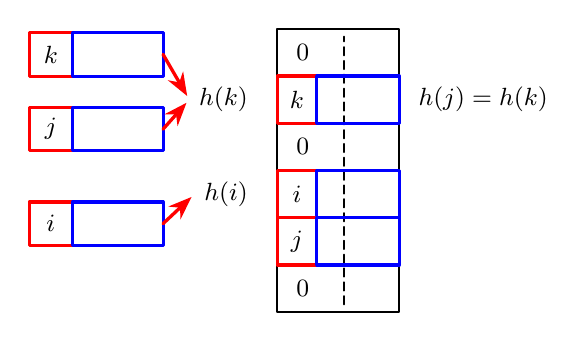
\begin{tikzpicture}[
					x=1cm,y=1cm,
					>=Stealth,
					line cap=round,line join=round,
					font=\small
					]
					%----- parameters
					\def\rowH{0.60}
					\def\tw{1.55}
					\def\th{3.60}
					\def\keyW{0.50}
					\def\valW{1.05}
					\def\dashX{0.85}
					
					% table bottom-left
					\coordinate (TBL) at (3.35,0.00);
					
					%----- draw table outer + row separators
					\draw[black, line width=0.8pt] (TBL) rectangle ++(\tw,\th);
					\foreach \r in {1,2,3,4,5}{
						\draw[black, line width=0.6pt]
						($(TBL)+(0,\r*\rowH)$) -- ($(TBL)+(\tw,\r*\rowH)$);
					}
					
					% dashed vertical line
					\draw[black, densely dashed, line width=0.7pt]
					($(TBL)+(\dashX,0.10)$) -- ($(TBL)+(\dashX,\th-0.10)$);
					
					%----- place 0's
					\node[anchor=west] at ($(TBL)+(0.12,5*\rowH+0.30)$) {$0$};
					\node[anchor=west] at ($(TBL)+(0.12,3*\rowH+0.30)$) {$0$};
					\node[anchor=west] at ($(TBL)+(0.12,0*\rowH+0.30)$) {$0$};
					
					%----- colored rows
					% row4: k
					\draw[red,  line width=1.1pt] ($(TBL)+(0,4*\rowH)$) rectangle ++(\keyW,\rowH);
					\draw[blue, line width=1.1pt] ($(TBL)+(\keyW,4*\rowH)$) rectangle ++(\valW,\rowH);
					\node at ($(TBL)+(\keyW/2,4*\rowH+0.30)$) {$k$};
					
					% row2: i
					\draw[red,  line width=1.1pt] ($(TBL)+(0,2*\rowH)$) rectangle ++(\keyW,\rowH);
					\draw[blue, line width=1.1pt] ($(TBL)+(\keyW,2*\rowH)$) rectangle ++(\valW,\rowH);
					\node at ($(TBL)+(\keyW/2,2*\rowH+0.30)$) {$i$};
					
					% row1: j
					\draw[red,  line width=1.1pt] ($(TBL)+(0,1*\rowH)$) rectangle ++(\keyW,\rowH);
					\draw[blue, line width=1.1pt] ($(TBL)+(\keyW,1*\rowH)$) rectangle ++(\valW,\rowH);
					\node at ($(TBL)+(\keyW/2,1*\rowH+0.30)$) {$j$};
					
					%===== labels h(k), h(i): arrows point to the TEXT
					\coordinate (hkLbl) at ($(TBL)+(-0.25,4*\rowH+0.30)$);
					\node[anchor=east] (hkNode) at (hkLbl) {$h(k)$};
					
					\coordinate (hiLbl) at ($(TBL)+(-0.25,2*\rowH+0.30)$);
					\node[anchor=east] (hiNode) at (hiLbl) {$h(i)$};
					
					% extra text on the right: h(j)=h(k)
					\node[anchor=west] at ($(TBL)+(\tw+0.12,4*\rowH+0.30)$) {$h(j)=h(k)$};
					
					%----- key boxes on the left (k, j, i)
					\def\bxX{0.20}
					\def\bxRedW{0.55}
					\def\bxBlueW{1.15}
					\def\bxH{0.55}
					
					% top: k
					\coordinate (B1) at (\bxX,3.00);
					\draw[red,  line width=1.1pt] (B1) rectangle ++(\bxRedW,\bxH);
					\draw[blue, line width=1.1pt] ($(B1)+(\bxRedW,0)$) rectangle ++(\bxBlueW,\bxH);
					\node at ($(B1)+(\bxRedW/2,\bxH/2)$) {$k$};
					\coordinate (kSrc) at ($(B1)+(\bxRedW+\bxBlueW, \bxH/2)$);
					
					% middle: j
					\coordinate (B2) at (\bxX,2.05);
					\draw[red,  line width=1.1pt] (B2) rectangle ++(\bxRedW,\bxH);
					\draw[blue, line width=1.1pt] ($(B2)+(\bxRedW,0)$) rectangle ++(\bxBlueW,\bxH);
					\node at ($(B2)+(\bxRedW/2,\bxH/2)$) {$j$};
					\coordinate (jSrc) at ($(B2)+(\bxRedW+\bxBlueW, \bxH/2)$);
					
					% bottom: i
					\coordinate (B3) at (\bxX,0.85);
					\draw[red,  line width=1.1pt] (B3) rectangle ++(\bxRedW,\bxH);
					\draw[blue, line width=1.1pt] ($(B3)+(\bxRedW,0)$) rectangle ++(\bxBlueW,\bxH);
					\node at ($(B3)+(\bxRedW/2,\bxH/2)$) {$i$};
					\coordinate (iSrc) at ($(B3)+(\bxRedW+\bxBlueW, \bxH/2)$);
					
					%----- arrows (to the TEXT)
					\draw[->, red, line width=1.2pt, shorten >=1.5pt] (kSrc) -- (hkNode.west);
					\draw[->, red, line width=1.2pt, shorten >=1.5pt] (jSrc) -- (hkNode.west);
					\draw[->, red, line width=1.2pt, shorten >=1.5pt] (iSrc) -- (hiNode.west);
					
				\end{tikzpicture}%
			}
		\end{column}
	\end{columns}
\end{frame}



%==================== SLIDE 31 ====================
\begin{frame}[t]{2. XUNG ĐỘT VÀ GIẢI QUYẾT XUNG ĐỘT}
	\small
	\setlength{\leftmargini}{-1.2em}
	
	\begin{itemize}
		\item Cách giải quyết xung đột bằng \textcolor{red}{phương pháp địa chỉ mở}:
		\begin{itemize}
			\item Khi bổ sung (\textit{Insert}): nếu ô là đã bận, thì ta tìm kiếm ô khác, \ldots, cho đến khi tìm được ô rỗng
			(\textit{phương pháp dò thử - probing}).
			
			\item Để tìm kiếm (\textit{search}), ta sẽ tìm dọc theo dãy các phép dò thử giống như dãy dò thử khi
			thực hiện chèn phần tử vào bảng.
			\begin{itemize}
				\item Nếu tìm được phần tử với khoá đã cho thì trả lại nó,
				\item Nếu tìm được con trỏ \texttt{NULL}, thì phần tử cần tìm không có trong bảng
			\end{itemize}
			
			\item Một số phương pháp dò:
			\begin{itemize}
				\item Dò tuyến tính (Linear Probing)
				\item Dò bậc hai (Quadratic Probing)
				\item Hàm băm kép (Double Hashing)
			\end{itemize}
		\end{itemize}
	\end{itemize}
\end{frame}


%==================== SLIDE 32 ====================
\begin{frame}[t]{2. XUNG ĐỘT VÀ GIẢI QUYẾT XUNG ĐỘT}
	\small
	\setlength{\leftmargini}{-1.2em}
	
	\begin{itemize}
		\item \textbf{Giải quyết xung đột bằng phương pháp địa chỉ mở}
		\begin{itemize}
			\item Phương pháp dò tuyến tính (Linear Probing):
			
			{\color{red}
				\item Mỗi lần dò, tăng chỉ số $i$ lên một đơn vị: $h(k,i) = (h'(k) + i)\ \mathrm{mod}\ p$ với $0 \le i \le p-1$
			}
			\vspace{-0.35em}
			\[
			h'(k) = k\ \mathrm{mod}\ p
			\]
			
		\end{itemize}
	\end{itemize}
	
	$\Rightarrow$ Đầu tiên thử $h(k,0)=h'(k)$, nếu vị trí này bận, thử tiếp $h(k,1)\ldots$ cho đến khi tìm được ô trống.
	
	\begin{center}
		\begin{tabular}{l}
			Lần băm 0: $h'(k)\ \mathrm{mod}\ p$\\[0.25em]
			Lần băm 1: $(h'(k)+1)\ \mathrm{mod}\ p$\\[0.25em]
			Lần băm 2: $(h'(k)+2)\ \mathrm{mod}\ p$\\[0.25em]
			Lần băm 3: $(h'(k)+3)\ \mathrm{mod}\ p$\\[0.25em]
			\ldots\\[0.25em]
			Lần băm $i$: $(h'(k)+i)\ \mathrm{mod}\ p$
		\end{tabular}
	\end{center}
\end{frame}

\begin{frame}[t]{2. XUNG ĐỘT VÀ GIẢI QUYẾT XUNG ĐỘT}
	\small
	\setlength{\leftmargini}{-1.2em}
	
	\begin{itemize}
		\item \textbf{Ví dụ: giải quyết xung đột bằng phương pháp địa chỉ mở}
		\begin{itemize}
			\item \textcolor{blue}{\textbf{Phương pháp dò tuyến tính}}
		\end{itemize}
	\end{itemize}
	
	\vspace{0.2cm}
	
	\begin{center}
		\begin{tabular}{@{}r l@{}}
			Sử dụng hàm băm: & $h'(k)=k\ \%\ 13$\\[0.65em]
			Chèn: &
			\tikz[remember picture,baseline=(k18.base)]
			\node[inner sep=0pt] (k18) {18,};
			\ 41,\ 22,\ 59,\ 32,\ 31,\ 73\\[0.65em]
			$h'(k)$: & 5,
		\end{tabular}
	\end{center}
	
	\vspace{0.55cm}
	
	\begin{center}
		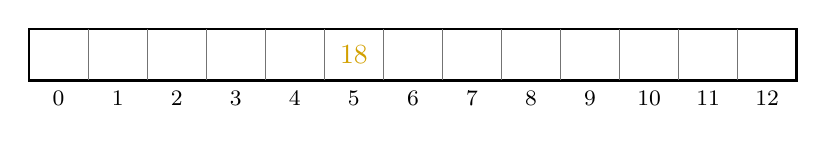
\begin{tikzpicture}[x=0.75cm,y=0.65cm,remember picture]
			\def\n{13}
			
			% Khung bảng
			\draw[line width=1pt] (0,0) rectangle (\n,1);
			\foreach \i in {1,...,12} {
				\draw[black!55] (\i,0) -- (\i,1);
			}
			
			% Ô index 5 chứa 18
			\node[font=\normalsize, text=codegold] (slot5) at (5.5,0.5) {18};
			\coordinate (top5) at (5.5,1);
			
			% Chỉ số 0..12
			\foreach \i in {0,...,12} {
				\node[font=\footnotesize] at (\i+0.5,-0.35) {\i};
			}
		\end{tikzpicture}
	\end{center}
	
	% Đường nối (không mũi tên) từ "18," xuống ô index 5
	\begin{tikzpicture}[remember picture,overlay]
		\draw[thin] (k18.south east) -- (top5);
	\end{tikzpicture}
	
\end{frame}

%========== Slide 34: chèn 41 ==========
\begin{frame}[t]{2. XUNG ĐỘT VÀ GIẢI QUYẾT XUNG ĐỘT}
	\small
	\setlength{\leftmargini}{-1.2em}
	
	\begin{itemize}
		\item \textbf{Ví dụ: giải quyết xung đột bằng phương pháp địa chỉ mở}
		\begin{itemize}
			\item \textcolor{blue}{\textbf{Phương pháp dò tuyến tính}}
		\end{itemize}
	\end{itemize}
	
	\vspace{0.2cm}
	
	\begin{center}
		\begin{tabular}{@{}r l@{}}
			Sử dụng hàm băm: & $h'(k)=k\ \%\ 13$\\[0.65em]
			Chèn: &
			18,\ 
			\tikz[remember picture,baseline=(k41s34.base)]
			\node[inner sep=0pt] (k41s34) {41,};
			\ 22,\ 59,\ 32,\ 31,\ 73\\[0.65em]
			$h'(k)$: & 5,\ \ 2,
		\end{tabular}
	\end{center}
	
	\vspace{0.55cm}
	
	\begin{center}
		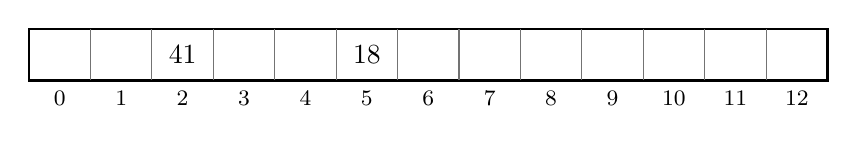
\begin{tikzpicture}[x=0.78cm,y=0.65cm,remember picture]
			\def\n{13}
			
			% Khung bảng
			\draw[line width=1pt] (0,0) rectangle (\n,1);
			\foreach \i in {1,...,12} { \draw[black!55] (\i,0) -- (\i,1); }
			
			% Giá trị trong bảng
			\node (s34slot2) at (2.5,0.5) {41};
			\node (s34slot5) at (5.5,0.5) {18};
			
			% Điểm neo để kẻ đường
			\coordinate (s34top2) at (2.5,1);
			
			% Chỉ số 0..12
			\foreach \i in {0,...,12} {
				\node[font=\footnotesize] at (\i+0.5,-0.35) {\i};
			}
		\end{tikzpicture}
	\end{center}
	
	% Đường nối tới ô 2
	\begin{tikzpicture}[remember picture,overlay]
		\draw[thin] (k41s34.south) -- (s34top2);
	\end{tikzpicture}
\end{frame}


%========== Slide 35: chèn 22 ==========
\begin{frame}[t]{2. XUNG ĐỘT VÀ GIẢI QUYẾT XUNG ĐỘT}
	\small
	\setlength{\leftmargini}{-1.2em}
	
	\begin{itemize}
		\item \textbf{Ví dụ: giải quyết xung đột bằng phương pháp địa chỉ mở}
		\begin{itemize}
			\item \textcolor{blue}{\textbf{Phương pháp dò tuyến tính}}
		\end{itemize}
	\end{itemize}
	
	\vspace{0.2cm}
	
	\begin{center}
		\begin{tabular}{@{}r l@{}}
			Sử dụng hàm băm: & $h'(k)=k\ \%\ 13$\\[0.65em]
			Chèn: &
			18,\ 41,\ 
			\tikz[remember picture,baseline=(k22s35.base)]
			\node[inner sep=0pt] (k22s35) {22,};
			\ 59,\ 32,\ 31,\ 73\\[0.65em]
			$h'(k)$: & 5,\ \ 2,\ \ 9
		\end{tabular}
	\end{center}
	
	\vspace{0.55cm}
	
	\begin{center}
		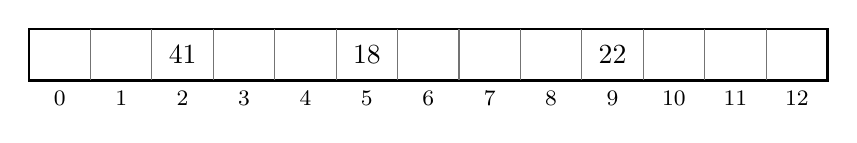
\begin{tikzpicture}[x=0.78cm,y=0.65cm,remember picture]
			\def\n{13}
			
			\draw[line width=1pt] (0,0) rectangle (\n,1);
			\foreach \i in {1,...,12} { \draw[black!55] (\i,0) -- (\i,1); }
			
			\node (s35slot2) at (2.5,0.5) {41};
			\node (s35slot5) at (5.5,0.5) {18};
			\node (s35slot9) at (9.5,0.5) {22};
			
			\coordinate (s35top9) at (9.5,1);
			
			\foreach \i in {0,...,12} {
				\node[font=\footnotesize] at (\i+0.5,-0.35) {\i};
			}
		\end{tikzpicture}
	\end{center}
	
	% Đường nối tới ô 9
	\begin{tikzpicture}[remember picture,overlay]
		\draw[thin] (k22s35.south) -- (s35top9);
	\end{tikzpicture}
\end{frame}


%========== Slide 36: chèn 59 ==========
\begin{frame}[t]{2. XUNG ĐỘT VÀ GIẢI QUYẾT XUNG ĐỘT}
	\small
	\setlength{\leftmargini}{-1.2em}
	
	\begin{itemize}
		\item \textbf{Ví dụ: giải quyết xung đột bằng phương pháp địa chỉ mở}
		\begin{itemize}
			\item \textcolor{blue}{\textbf{Phương pháp dò tuyến tính}}
		\end{itemize}
	\end{itemize}
	
	\vspace{0.2cm}
	
	\begin{center}
		\begin{tabular}{@{}r l@{}}
			Sử dụng hàm băm: & $h'(k)=k\ \%\ 13$\\[0.65em]
			Chèn: &
			18,\ 41,\ 22,\ 
			\tikz[remember picture,baseline=(k59s36.base)]
			\node[inner sep=0pt] (k59s36) {59,};
			\ 32,\ 31,\ 73\\[0.65em]
			$h'(k)$: & 5,\ \ 2,\ \ 9,\ \ 7,
		\end{tabular}
	\end{center}
	
	\vspace{0.55cm}
	
	\begin{center}
		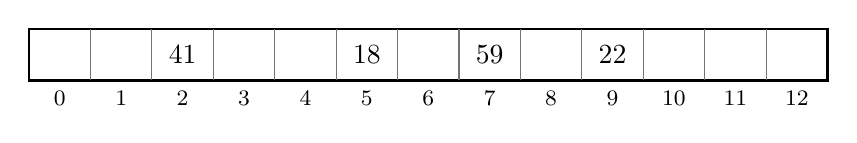
\begin{tikzpicture}[x=0.78cm,y=0.65cm,remember picture]
			\def\n{13}
			
			\draw[line width=1pt] (0,0) rectangle (\n,1);
			\foreach \i in {1,...,12} { \draw[black!55] (\i,0) -- (\i,1); }
			
			\node (s36slot2) at (2.5,0.5) {41};
			\node (s36slot5) at (5.5,0.5) {18};
			\node (s36slot7) at (7.5,0.5) {59};
			\node (s36slot9) at (9.5,0.5) {22};
			
			\coordinate (s36top7) at (7.5,1);
			
			\foreach \i in {0,...,12} {
				\node[font=\footnotesize] at (\i+0.5,-0.35) {\i};
			}
		\end{tikzpicture}
	\end{center}
	
	% Đường nối tới ô 7
	\begin{tikzpicture}[remember picture,overlay]
		\draw[thin] (k59s36.south) -- (s36top7);
	\end{tikzpicture}
\end{frame}

\begin{frame}[t]{2. XUNG ĐỘT VÀ GIẢI QUYẾT XUNG ĐỘT}
	\small
	\setlength{\leftmargini}{-1.2em}
	
	\begin{itemize}
		\item \textbf{Ví dụ: giải quyết xung đột bằng phương pháp địa chỉ mở}
		\begin{itemize}
			\item \textcolor{blue}{\textbf{Phương pháp dò tuyến tính}}
		\end{itemize}
	\end{itemize}
	
	\vspace{0.25cm}
	
	\begin{center}
		\begin{tabular}{@{}r l@{}}
			Sử dụng hàm băm: & $h'(k)=k\ \%\ 13$\\[0.9em]
			Chèn: &
			18,\ \ 41,\ \ 22,\ \ 59,\ \
			\tikz[remember picture,baseline=(k32.base)]
			\node[inner sep=0pt,outer sep=0pt] (k32) {32};,%
			\ \ 31,\ \ 73\\[0.9em]
			$h'(k)$: & 5,\ \ 2,\ \ 9,\ \ 7,\ \ 6,
		\end{tabular}
	\end{center}
	
	\vspace{0.65cm}
	
	\begin{center}
		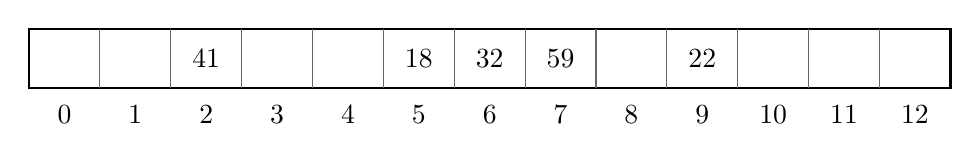
\begin{tikzpicture}[x=0.9cm,y=0.75cm,remember picture]
			\def\n{13}
			
			% bảng băm
			\draw[line width=1pt] (0,0) rectangle (\n,1);
			\foreach \i in {1,...,12} { \draw[black!60] (\i,0) -- (\i,1); }
			
			% các giá trị đã chèn
			\node at (2.5,0.5) {41};
			\node at (5.5,0.5) {18};
			\node at (6.5,0.5) {32};
			\node at (7.5,0.5) {59};
			\node at (9.5,0.5) {22};
			
			% điểm neo để kẻ đường tới ô 6
			\coordinate (top6) at (6.5,1);
			
			% chỉ số 0..12
			\foreach \i in {0,...,12} {
				\node[font=\normalsize] at (\i+0.5,-0.45) {\i};
			}
		\end{tikzpicture}
	\end{center}
	
	% đường nối từ "32" xuống ô 6 (không mũi tên), đặt đúng dưới số 32
	\begin{tikzpicture}[remember picture,overlay]
		\draw[thin] ([yshift=-1.5pt]k32.south) -- (top6);
	\end{tikzpicture}
\end{frame}


%========== Slide 38: chèn 31 (31%13=5, dò tuyến tính tới ô 8) ==========
\begin{frame}[t]{2. XUNG ĐỘT VÀ GIẢI QUYẾT XUNG ĐỘT}
	\small
	\setlength{\leftmargini}{-1.2em}
	
	\begin{itemize}
		\item \textbf{Ví dụ: giải quyết xung đột bằng phương pháp địa chỉ mở}
		\begin{itemize}
			\item \textcolor{blue}{\textbf{Phương pháp dò tuyến tính}}
		\end{itemize}
	\end{itemize}
	
	\vspace{0.2cm}
	
	\begin{center}
		\begin{tabular}{@{}r l@{}}
			Sử dụng hàm băm: & $h'(k)=k\ \%\ 13$\\[0.65em]
			Chèn: &
			18,\ 41,\ 22,\ 59,\ 32,\ 
			\tikz[remember picture,baseline=(k31s38.base)]
			\node[inner sep=0pt,outer sep=0pt] (k31s38) {31};, %
			\ 73\\[0.65em]
			$h'(k)$: & 5,\ \ 2,\ \ 9,\ \ 7,\ \ 6,\ \ 5,
		\end{tabular}
	\end{center}
	
	\vspace{0.55cm}
	
	\begin{center}
		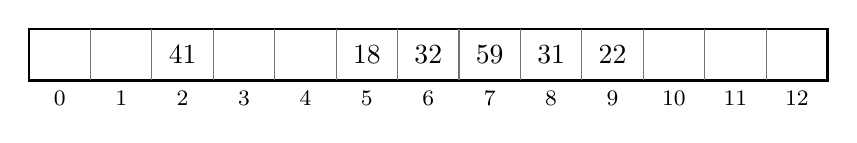
\begin{tikzpicture}[x=0.78cm,y=0.65cm,remember picture]
			\def\n{13}
			
			\draw[line width=1pt] (0,0) rectangle (\n,1);
			\foreach \i in {1,...,12} { \draw[black!55] (\i,0) -- (\i,1); }
			
			\node at (2.5,0.5) {41};
			\node at (5.5,0.5) {18};
			\node at (6.5,0.5) {32};
			\node at (7.5,0.5) {59};
			\node at (8.5,0.5) {31};
			\node at (9.5,0.5) {22};
			
			\coordinate (s38top8) at (8.5,1);
			
			\foreach \i in {0,...,12} {
				\node[font=\footnotesize] at (\i+0.5,-0.35) {\i};
			}
		\end{tikzpicture}
	\end{center}
	
	\begin{tikzpicture}[remember picture,overlay]
		\draw[thin] ([yshift=-1.5pt]k31s38.south) -- (s38top8);
	\end{tikzpicture}
\end{frame}


%========== Slide 39: chèn 73 (73%13=8, dò tuyến tính tới ô 10) ==========
\begin{frame}[t]{2. XUNG ĐỘT VÀ GIẢI QUYẾT XUNG ĐỘT}
	\small
	\setlength{\leftmargini}{-1.2em}
	
	\begin{itemize}
		\item \textbf{Ví dụ: giải quyết xung đột bằng phương pháp địa chỉ mở}
		\begin{itemize}
			\item \textcolor{blue}{\textbf{Phương pháp dò tuyến tính}}
		\end{itemize}
	\end{itemize}
	
	\vspace{0.2cm}
	
	\begin{center}
		\begin{tabular}{@{}r l@{}}
			Sử dụng hàm băm: & $h'(k)=k\ \%\ 13$\\[0.65em]
			Chèn: &
			18,\ 41,\ 22,\ 59,\ 32,\ 31,\ 
			\tikz[remember picture,baseline=(k73s39.base)]
			\node[inner sep=0pt,outer sep=0pt] (k73s39) {73};\\[0.65em]
			$h'(k)$: & 5,\ \ 2,\ \ 9,\ \ 7,\ \ 6,\ \ 5,\ \ 8
		\end{tabular}
	\end{center}
	
	\vspace{0.55cm}
	
	\begin{center}
		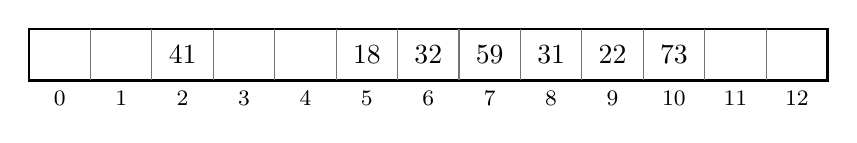
\begin{tikzpicture}[x=0.78cm,y=0.65cm,remember picture]
			\def\n{13}
			
			\draw[line width=1pt] (0,0) rectangle (\n,1);
			\foreach \i in {1,...,12} { \draw[black!55] (\i,0) -- (\i,1); }
			
			\node at (2.5,0.5) {41};
			\node at (5.5,0.5) {18};
			\node at (6.5,0.5) {32};
			\node at (7.5,0.5) {59};
			\node at (8.5,0.5) {31};
			\node at (9.5,0.5) {22};
			\node at (10.5,0.5) {73};
			
			\coordinate (s39top10) at (10.5,1);
			
			\foreach \i in {0,...,12} {
				\node[font=\footnotesize] at (\i+0.5,-0.35) {\i};
			}
		\end{tikzpicture}
	\end{center}
	
	\begin{tikzpicture}[remember picture,overlay]
		\draw[thin] ([yshift=-1.5pt]k73s39.south) -- (s39top10);
	\end{tikzpicture}
\end{frame}

\begin{frame}[t]{2. XUNG ĐỘT VÀ GIẢI QUYẾT XUNG ĐỘT}
	\small
	\setlength{\leftmargini}{-1.2em}
	
	\begin{itemize}
		\item \textbf{Ví dụ: giải quyết xung đột bằng phương pháp địa chỉ mở}
		\begin{itemize}
			\item \textcolor{blue}{\textbf{Phương pháp dò tuyến tính}}
		\end{itemize}
	\end{itemize}
	
	\vspace{0.25cm}
	
	\begin{center}
		\begin{tabular}{@{}r l@{}}
			Sử dụng hàm băm: & $h'(k)=k\ \%\ 13$\\[0.9em]
			Chèn: &
			18,\ 41,\ 22,\ 59,\ 32,\ 
			\tikz[remember picture,baseline=(k31.base)]
			\node[inner sep=0pt,outer sep=0pt] (k31) {31};,%
			\ 73\\[0.9em]
			$h'(k)$: & 5,\ \ 2,\ \ 9,\ \ 7,\ \ 6,\ \ 5,
		\end{tabular}
	\end{center}
	
	\vspace{0.6cm}
	
	\begin{center}
		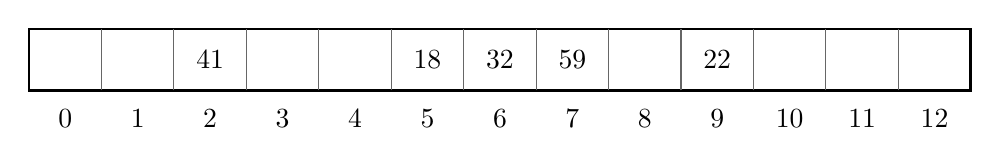
\begin{tikzpicture}[x=0.92cm,y=0.78cm,remember picture]
			\def\n{13}
			
			% bảng băm
			\draw[line width=1pt] (0,0) rectangle (\n,1);
			\foreach \i in {1,...,12} { \draw[black!60] (\i,0) -- (\i,1); }
			
			% các giá trị đã chèn (chưa chèn 31)
			\node at (2.5,0.5) {41};
			\node at (5.5,0.5) {18};
			\node at (6.5,0.5) {32};
			\node at (7.5,0.5) {59};
			\node at (9.5,0.5) {22};
			
			% điểm neo để kẻ mũi tên tới ô 5 (đang bị chiếm bởi 18)
			\coordinate (top5) at (5.5,1);
			
			% chỉ số 0..12
			\foreach \i in {0,...,12} {
				\node[font=\normalsize] at (\i+0.5,-0.45) {\i};
			}
		\end{tikzpicture}
		\end{center}
		
		% mũi tên + 2 hộp mô tả bên phải
		\begin{tikzpicture}[remember picture,overlay]
		% ---- chỉnh nhanh kích thước ở đây ----
		\def\AWIDTH{0.30\textwidth} % khung trên
		\def\BWIDTH{0.22\textwidth} % khung dưới (THU HẸP Ở ĐÂY)
		% -------------------------------------
		
		% mũi tên từ "31" tới vị trí băm đầu tiên (ô 5)
		\draw[-{Stealth[length=2.6mm,width=1.8mm]},thin]
		([yshift=-1.5pt]k31.south) -- (top5);
		
		% ====== BOX 1 (công thức) ======
		\node[
		anchor=north east,
		draw=codeblue,
		text=codeblue,
		line width=0.6pt,
		inner xsep=4pt, inner ysep=3pt,
		text width=\AWIDTH,
		align=left,
		font=\tiny
		] (boxA) at ([xshift=-0.25cm,yshift=-1.55cm]current page.north east)
		{%
			{\linespread{0.85}\selectfont
				Lần băm 0: $h'(k)\bmod m$\par
				Lần băm 1: $(h'(k)+1)\bmod m$\par
				Lần băm 2: $(h'(k)+2)\bmod m$\par
				Lần băm 3: $(h'(k)+3)\bmod m$\par
				$\dots$\par
				Lần băm $i$: $(h'(k)+i)\bmod m$
			}
		};
		
		% ====== BOX 2 (mô tả) ======
		\node[
		anchor=north east,
		draw=codeblue,
		text=codeblue,
		line width=0.6pt,
		inner xsep=4pt, inner ysep=3pt,
		text width=\BWIDTH,
		align=left,
		font=\tiny
		] at ([yshift=-0.22cm]boxA.south east)
		{%
			{\linespread{0.85}\selectfont
				\textbf{Đầu tiên thử} $h(k,0)=h'(k)$, nếu vị trí này bận, thử tiếp $h(k,1)$, ... cho đến khi tìm được ô trống.
			}
		};
		\end{tikzpicture}
\end{frame}

\begin{frame}[t]{2. XUNG ĐỘT VÀ GIẢI QUYẾT XUNG ĐỘT}
	\small
	\setlength{\leftmargini}{-1.2em}
	
	\begin{itemize}
		\item \textbf{Ví dụ: giải quyết xung đột bằng phương pháp địa chỉ mở}
		\begin{itemize}
			\item \textcolor{blue}{\textbf{Phương pháp dò tuyến tính}}
		\end{itemize}
	\end{itemize}
	
	\vspace{0.35cm}
	
	\begin{center}
		{\large Sử dụng hàm băm: $h'(k)=k\ \%\ 13$}\\[0.45cm]
		
		{\Large
			Chèn:\quad 18,\ 41,\ 22,\ 59,\ 32,\ 
			\tikz[remember picture,baseline=(k31.base)]
			\node[inner sep=0pt,outer sep=0pt] (k31) {31};,
			\ 73
		}\\[0.40cm]
		
		{\Large $h'(k)$:\quad 5,\ 2,\ 9,\ 7,\ 6,\ 5,}
	\end{center}
	
	\vspace{0.55cm}
	
	\begin{center}
		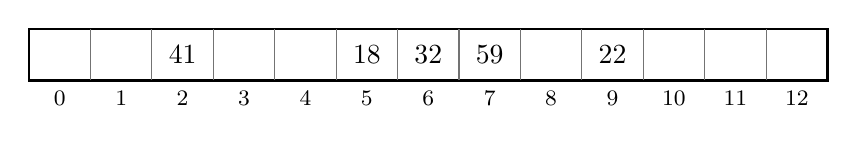
\begin{tikzpicture}[x=0.78cm,y=0.65cm,remember picture]
			\def\n{13}
			
			% bảng băm
			\draw[line width=1pt] (0,0) rectangle (\n,1);
			\foreach \i in {1,...,12} { \draw[black!55] (\i,0) -- (\i,1); }
			
			% trạng thái hiện tại (chưa chèn 31)
			\node at (2.5,0.5) {41};
			\node at (5.5,0.5) {18};
			\node at (6.5,0.5) {32};
			\node at (7.5,0.5) {59};
			\node at (9.5,0.5) {22};
			
			% điểm để vẽ đường và mũi tên cong (dò tuyến tính 5 -> 6)
			\coordinate (probeFrom) at (5.55,1.05);
			\coordinate (probeTo)   at (6.55,1.05);
			
			% chỉ số 0..12
			\foreach \i in {0,...,12} {
				\node[font=\footnotesize] at (\i+0.5,-0.35) {\i};
			}
		\end{tikzpicture}
	\end{center}
	
	\begin{tikzpicture}[remember picture,overlay]
		% đường chéo từ "31" xuống vùng dò (không mũi tên)
		\draw[thin] ([yshift=-1.5pt]k31.south) -- (probeFrom);
		
		% mũi tên cong nhỏ vừa như ảnh (viền đen + ruột xanh)
		\draw[-{Stealth[length=3.6mm,width=4.2mm]}, line width=3.0pt, draw=black]
		(probeFrom) to[bend left=45] (probeTo);
		\draw[-{Stealth[length=3.6mm,width=4.2mm]}, line width=2.1pt, draw=codeblue!80]
		(probeFrom) to[bend left=45] (probeTo);
	\end{tikzpicture}
	
\end{frame}

%==================== Slide 40: chèn 31 (dò 5 -> 6 -> 7) ====================
\begin{frame}[t]{2. XUNG ĐỘT VÀ GIẢI QUYẾT XUNG ĐỘT}
	\small
	\setlength{\leftmargini}{-1.2em}
	
	\begin{itemize}
		\item \textbf{Ví dụ: giải quyết xung đột bằng phương pháp địa chỉ mở}
		\begin{itemize}
			\item \textcolor{blue}{\textbf{Phương pháp dò tuyến tính}}
		\end{itemize}
	\end{itemize}
	
	\vspace{0.2cm}
	
	\begin{center}
		\begin{tabular}{@{}r l@{}}
			Sử dụng hàm băm: & $h'(k)=k\ \%\ 13$\\[0.65em]
			Chèn: &
			18,\ 41,\ 22,\ 59,\ 32,\ 
			\tikz[remember picture,baseline=(k31s40.base)]
			\node[inner sep=0pt,outer sep=0pt] (k31s40) {31};,\ \ 73\\[0.65em]
			$h'(k)$: & 5,\ \ 2,\ \ 9,\ \ 7,\ \ 6,\ \ 5,
		\end{tabular}
	\end{center}
	
	\vspace{0.55cm}
	
	\begin{center}
		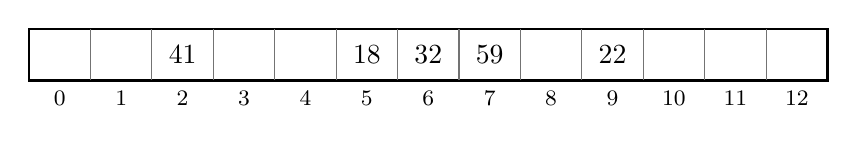
\begin{tikzpicture}[x=0.78cm,y=0.65cm,remember picture]
			\def\n{13}
			
			% bảng băm
			\draw[line width=1pt] (0,0) rectangle (\n,1);
			\foreach \i in {1,...,12} { \draw[black!55] (\i,0) -- (\i,1); }
			
			% trạng thái hiện tại (chưa đặt 31)
			\node at (2.5,0.5) {41};
			\node at (5.5,0.5) {18};
			\node at (6.5,0.5) {32};
			\node at (7.5,0.5) {59};
			\node at (9.5,0.5) {22};
			
			% điểm cho mũi tên cong dò tuyến tính
			\coordinate (p56a) at (5.55,1.05);
			\coordinate (p56b) at (6.55,1.05);
			\coordinate (p67a) at (6.55,1.05);
			\coordinate (p67b) at (7.55,1.05);
			
			% chỉ số 0..12
			\foreach \i in {0,...,12} {
				\node[font=\footnotesize] at (\i+0.5,-0.35) {\i};
			}
		\end{tikzpicture}
	\end{center}
	
	\begin{tikzpicture}[remember picture,overlay]
		% đường chỉ từ "31" xuống vùng dò
		\draw[thin] ([yshift=-1.5pt]k31s40.south) -- (p56a);
		
		% mũi tên cong 5->6 (viền đen + ruột xanh)
		\draw[-{Stealth[length=3.6mm,width=4.2mm]}, line width=3.0pt, draw=black]
		(p56a) to[bend left=55] (p56b);
		\draw[-{Stealth[length=3.6mm,width=4.2mm]}, line width=2.1pt, draw=codeblue!80]
		(p56a) to[bend left=55] (p56b);
		
		% mũi tên cong 6->7 (viền đen + ruột xanh)
		\draw[-{Stealth[length=3.6mm,width=4.2mm]}, line width=3.0pt, draw=black]
		(p67a) to[bend left=55] (p67b);
		\draw[-{Stealth[length=3.6mm,width=4.2mm]}, line width=2.1pt, draw=codeblue!80]
		(p67a) to[bend left=55] (p67b);
	\end{tikzpicture}
\end{frame}


%==================== Slide 41: chèn 31 (dò 5 -> 6 -> 7 -> 8, đặt ở 8) ====================
\begin{frame}[t]{2. XUNG ĐỘT VÀ GIẢI QUYẾT XUNG ĐỘT}
	\small
	\setlength{\leftmargini}{-1.2em}
	
	\begin{itemize}
		\item \textbf{Ví dụ: giải quyết xung đột bằng phương pháp địa chỉ mở}
		\begin{itemize}
			\item \textcolor{blue}{\textbf{Phương pháp dò tuyến tính}}
		\end{itemize}
	\end{itemize}
	
	\vspace{0.2cm}
	
	\begin{center}
		\begin{tabular}{@{}r l@{}}
			Sử dụng hàm băm: & $h'(k)=k\ \%\ 13$\\[0.65em]
			Chèn: &
			18,\ 41,\ 22,\ 59,\ 32,\ 
			\tikz[remember picture,baseline=(k31s41.base)]
			\node[inner sep=0pt,outer sep=0pt] (k31s41) {31};,\ \ 73\\[0.65em]
			$h'(k)$: & 5,\ \ 2,\ \ 9,\ \ 7,\ \ 6,\ \ 5,
		\end{tabular}
	\end{center}
	
	\vspace{0.55cm}
	
	\begin{center}
		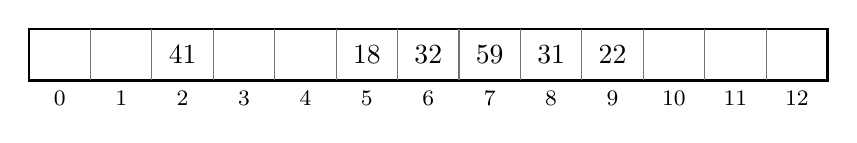
\begin{tikzpicture}[x=0.78cm,y=0.65cm,remember picture]
			\def\n{13}
			
			% bảng băm
			\draw[line width=1pt] (0,0) rectangle (\n,1);
			\foreach \i in {1,...,12} { \draw[black!55] (\i,0) -- (\i,1); }
			
			% trạng thái sau khi đặt 31 ở ô 8
			\node at (2.5,0.5) {41};
			\node at (5.5,0.5) {18};
			\node at (6.5,0.5) {32};
			\node at (7.5,0.5) {59};
			\node at (8.5,0.5) {31};
			\node at (9.5,0.5) {22};
			
			% điểm cho mũi tên cong dò tuyến tính
			\coordinate (p56a) at (5.55,1.05);
			\coordinate (p56b) at (6.55,1.05);
			\coordinate (p67a) at (6.55,1.05);
			\coordinate (p67b) at (7.55,1.05);
			\coordinate (p78a) at (7.55,1.05);
			\coordinate (p78b) at (8.55,1.05);
			
			% chỉ số 0..12
			\foreach \i in {0,...,12} {
				\node[font=\footnotesize] at (\i+0.5,-0.35) {\i};
			}
		\end{tikzpicture}
	\end{center}
	
	\begin{tikzpicture}[remember picture,overlay]
		% đường chỉ từ "31" xuống vùng dò
		\draw[thin] ([yshift=-1.5pt]k31s41.south) -- (p56a);
		
		% 5->6
		\draw[-{Stealth[length=3.6mm,width=4.2mm]}, line width=3.0pt, draw=black]
		(p56a) to[bend left=55] (p56b);
		\draw[-{Stealth[length=3.6mm,width=4.2mm]}, line width=2.1pt, draw=codeblue!80]
		(p56a) to[bend left=55] (p56b);
		
		% 6->7
		\draw[-{Stealth[length=3.6mm,width=4.2mm]}, line width=3.0pt, draw=black]
		(p67a) to[bend left=55] (p67b);
		\draw[-{Stealth[length=3.6mm,width=4.2mm]}, line width=2.1pt, draw=codeblue!80]
		(p67a) to[bend left=55] (p67b);
		
		% 7->8
		\draw[-{Stealth[length=3.6mm,width=4.2mm]}, line width=3.0pt, draw=black]
		(p78a) to[bend left=55] (p78b);
		\draw[-{Stealth[length=3.6mm,width=4.2mm]}, line width=2.1pt, draw=codeblue!80]
		(p78a) to[bend left=55] (p78b);
	\end{tikzpicture}
\end{frame}

\begin{frame}[t]{2. XUNG ĐỘT VÀ GIẢI QUYẾT XUNG ĐỘT}
	\small
	\setlength{\leftmargini}{-1.2em}
	\definecolor{codeblue}{RGB}{0,90,200}
	
	\begin{itemize}
		\item \textbf{Ví dụ: giải quyết xung đột bằng phương pháp địa chỉ mở}
		\begin{itemize}
			\item \textcolor{blue}{\textbf{Phương pháp dò tuyến tính}}
		\end{itemize}
	\end{itemize}
	
	\vspace{0.25cm}
	
	\begin{center}
		\begin{tabular}{@{}r l@{}}
			Sử dụng hàm băm: & $h'(k)=k\ \%\ 13$\\[0.9em]
			Chèn: &
			18,\ 41,\ 22,\ 59,\ 32,\ 31,\ 
			\tikz[remember picture,baseline=(k73.base)]
			\node[inner sep=0pt,outer sep=0pt] (k73) {73};\\[0.9em]
			$h'(k)$: & 5,\ \ 2,\ \ 9,\ \ 7,\ \ 6,\ \ 5,\ \ 8
		\end{tabular}
	\end{center}
	
	\vspace{0.6cm}
	
	\begin{center}
		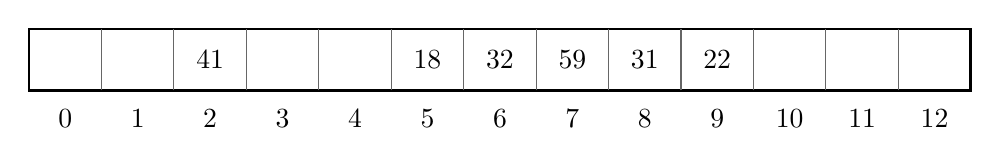
\begin{tikzpicture}[x=0.92cm,y=0.78cm,remember picture]
			\def\n{13}
			
			% bảng băm
			\draw[line width=1pt] (0,0) rectangle (\n,1);
			\foreach \i in {1,...,12} { \draw[black!60] (\i,0) -- (\i,1); }
			
			% các giá trị đã chèn (đã có 31 ở ô 8, CHƯA chèn 73)
			\node at (2.5,0.5) {41};   % index 2
			\node at (5.5,0.5) {18};   % index 5
			\node at (6.5,0.5) {32};   % index 6
			\node at (7.5,0.5) {59};   % index 7
			\node at (8.5,0.5) {31};   % index 8
			\node at (9.5,0.5) {22};   % index 9
			
			% điểm neo để kẻ mũi tên tới ô 8 (h'(73)=8, đang bị chiếm bởi 31)
			\coordinate (top8) at (8.5,1);
			
			% chỉ số 0..12
			\foreach \i in {0,...,12} {
				\node[font=\normalsize] at (\i+0.5,-0.45) {\i};
			}
		\end{tikzpicture}
	\end{center}
	
	% mũi tên + 2 hộp mô tả bên phải
	\begin{tikzpicture}[remember picture,overlay]
		% ---- chỉnh nhanh kích thước ở đây ----
		\def\AWIDTH{0.30\textwidth} % khung trên
		\def\BWIDTH{0.22\textwidth} % khung dưới
		% -------------------------------------
		
		% mũi tên từ "73" tới vị trí băm đầu tiên (ô 8)
		\draw[-{Stealth[length=2.6mm,width=1.8mm]},thin]
		([yshift=-1.5pt]k73.south) -- (top8);
		
		% ====== BOX 1 (công thức) ======
		\node[
		anchor=north east,
		draw=codeblue,
		text=codeblue,
		line width=0.6pt,
		inner xsep=4pt, inner ysep=3pt,
		text width=\AWIDTH,
		align=left,
		font=\tiny
		] (boxA) at ([xshift=-0.25cm,yshift=-1.55cm]current page.north east)
		{%
			{\linespread{0.85}\selectfont
				Lần băm 0: $h'(k)\bmod m$\par
				Lần băm 1: $(h'(k)+1)\bmod m$\par
				Lần băm 2: $(h'(k)+2)\bmod m$\par
				Lần băm 3: $(h'(k)+3)\bmod m$\par
				$\dots$\par
				Lần băm $i$: $(h'(k)+i)\bmod m$
			}
		};
		
		% ====== BOX 2 (mô tả) ======
		\node[
		anchor=north east,
		draw=codeblue,
		text=codeblue,
		line width=0.6pt,
		inner xsep=4pt, inner ysep=3pt,
		text width=\BWIDTH,
		align=left,
		font=\tiny
		] at ([yshift=-0.22cm]boxA.south east)
		{%
			{\linespread{0.85}\selectfont
				\textbf{Đầu tiên thử} $h(k,0)=h'(k)$, nếu vị trí này bận, thử tiếp $h(k,1)$, ... cho đến khi tìm được ô trống.
			}
		};
	\end{tikzpicture}
\end{frame}

\begin{frame}[t]{2. XUNG ĐỘT VÀ GIẢI QUYẾT XUNG ĐỘT}
	\small
	\setlength{\leftmargini}{-1.2em}
	
	\begin{itemize}
		\item \textbf{Ví dụ: giải quyết xung đột bằng phương pháp địa chỉ mở}
		\begin{itemize}
			\item \textcolor{blue}{\textbf{Phương pháp dò tuyến tính}}
		\end{itemize}
	\end{itemize}
	
	\vspace{0.25cm}
	
	\begin{center}
		\begin{tabular}{@{}r l@{}}
			Sử dụng hàm băm: & $h'(k)=k\ \%\ 13$\\[0.9em]
			Chèn: &
			18,\ 41,\ 22,\ 59,\ 32,\ 31,\ 
			\tikz[remember picture,baseline=(k73.base)]
			\node[inner sep=0pt,outer sep=0pt] (k73) {73};\\[0.9em]
			$h'(k)$: & 5,\ \ 2,\ \ 9,\ \ 7,\ \ 6,\ \ 5,\ \ 8
		\end{tabular}
	\end{center}
	
	\vspace{0.6cm}
	
	\begin{center}
		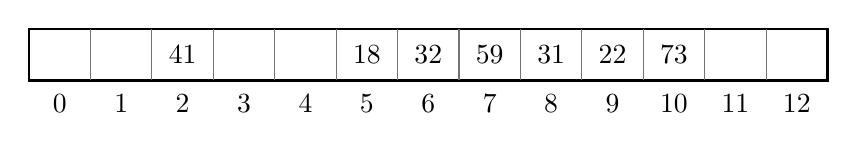
\begin{tikzpicture}[x=0.78cm,y=0.65cm,remember picture]
			\def\n{13}
			
			% bảng băm
			\draw[line width=1pt] (0,0) rectangle (\n,1);
			\foreach \i in {1,...,12} { \draw[black!55] (\i,0) -- (\i,1); }
			
			% trạng thái SAU khi chèn 73 (vào ô 10)
			\node at (2.5,0.5)  {41};
			\node at (5.5,0.5)  {18};
			\node at (6.5,0.5)  {32};
			\node at (7.5,0.5)  {59};
			\node at (8.5,0.5)  {31};
			\node at (9.5,0.5)  {22};
			\node at (10.5,0.5) {73};
			
			% điểm cho mũi tên cong dò tuyến tính 8->9->10
			\coordinate (p89a)  at (8.55,1.05);
			\coordinate (p89b)  at (9.55,1.05);
			\coordinate (p910a) at (9.55,1.05);
			\coordinate (p910b) at (10.55,1.05);
			
			% chỉ số 0..12 (to như hình)
			\foreach \i in {0,...,12} {
				\node[font=\normalsize] at (\i+0.5,-0.45) {\i};
			}
		\end{tikzpicture}
	\end{center}
	
	% mũi tên + 2 hộp mô tả bên phải
	\begin{tikzpicture}[remember picture,overlay]
		% ---- kích thước 2 khung như slide hiện tại ----
		\def\AWIDTH{0.30\textwidth}
		\def\BWIDTH{0.22\textwidth}
		
		% đường chỉ từ "73" xuống vùng dò (không mũi tên)
		\draw[thin] ([yshift=-1.5pt]k73.south) -- (p89a);
		
		% mũi tên cong 8->9 (viền đen + ruột xanh)
		\draw[-{Stealth[length=3.6mm,width=4.2mm]}, line width=3.0pt, draw=black]
		(p89a) to[bend left=55] (p89b);
		\draw[-{Stealth[length=3.6mm,width=4.2mm]}, line width=2.1pt, draw=codeblue!80]
		(p89a) to[bend left=55] (p89b);
		
		% mũi tên cong 9->10 (viền đen + ruột xanh)
		\draw[-{Stealth[length=3.6mm,width=4.2mm]}, line width=3.0pt, draw=black]
		(p910a) to[bend left=55] (p910b);
		\draw[-{Stealth[length=3.6mm,width=4.2mm]}, line width=2.1pt, draw=codeblue!80]
		(p910a) to[bend left=55] (p910b);
		
		% ====== BOX 1 (công thức) ======
		\node[
		anchor=north east,
		draw=codeblue,
		text=codeblue,
		line width=0.6pt,
		inner xsep=4pt, inner ysep=3pt,
		text width=\AWIDTH,
		align=left,
		font=\tiny
		] (boxA) at ([xshift=-0.25cm,yshift=-1.55cm]current page.north east)
		{%
			{\linespread{0.85}\selectfont
				Lần băm 0: $h'(k)\bmod m$\par
				Lần băm 1: $(h'(k)+1)\bmod m$\par
				Lần băm 2: $(h'(k)+2)\bmod m$\par
				Lần băm 3: $(h'(k)+3)\bmod m$\par
				$\dots$\par
				Lần băm $i$: $(h'(k)+i)\bmod m$
			}
		};
		
		% ====== BOX 2 (mô tả) ======
		\node[
		anchor=north east,
		draw=codeblue,
		text=codeblue,
		line width=0.6pt,
		inner xsep=4pt, inner ysep=3pt,
		text width=\BWIDTH,
		align=left,
		font=\tiny
		] at ([yshift=-0.22cm]boxA.south east)
		{%
			{\linespread{0.85}\selectfont
				\textbf{Đầu\qquad tiên\qquad thử}\par
				$h(k,0)=h'(k)$, nếu vị trí này bận, thử tiếp $h(k,1)$... cho đến khi tìm được ô trống.
			}
		};
	\end{tikzpicture}
\end{frame}

% =========================================================
% SLIDE 44 — Quadratic Probing (đúng size + đúng bố cục)
% =========================================================
\begin{frame}[t]{2. XUNG ĐỘT VÀ GIẢI QUYẾT XUNG ĐỘT}
	\small
	\setlength{\leftmargini}{-1.2em}
	\definecolor{hashBlue}{RGB}{0,70,140}
	
	\begin{itemize}
		\item \textbf{Giải quyết xung đột bằng phương pháp địa chỉ mở}
	\end{itemize}
	
	\begin{itemize}
		\item[\textcolor{hashBlue}{\Large\textbullet}] \textbf{Phương pháp dò bậc hai (Quadratic Probing):}
	\end{itemize}
	
	\vspace{0.05cm}
	
	\begin{itemize}
		\item[\textcolor{red}{\Large\textbullet}] \textcolor{red}{\textbf{Mỗi lần dò, tăng chỉ số $i$ lên bình phương:}}
	\end{itemize}
	
	\hspace*{1.15cm}
	{\color{red}$
		h(k,i)=(h'(k)+i^2)\ \mathrm{mod}\ p
		\ \text{với}\ 0\le i\le p-1;\quad
		h'(k)=k\ \mathrm{mod}\ p
		$}
	
	\hspace*{0.60cm}
	\\
	$\Rightarrow$ Đầu tiên thử $h(k,0)=h'(k)$, nếu vị trí này bận, thử tiếp $h(k,1)$... cho đến khi tìm được ô trống.
	
	\hspace*{3.20cm}Lần băm 0:\ \ $h'(k)\ \mathrm{mod}\ p$\\[0.05cm]
	\hspace*{3.20cm}Lần băm 1:\ \ $(h'(k)+1)\ \mathrm{mod}\ p$\\[0.05cm]
	\hspace*{3.20cm}Lần băm 2:\ \ $(h'(k)+4)\ \mathrm{mod}\ p$\\[0.05cm]
	\hspace*{3.20cm}Lần băm 3:\ \ $(h'(k)+9)\ \mathrm{mod}\ p$\\[0.05cm]
	\hspace*{3.20cm}\ldots\\[0.05cm]
	\hspace*{3.20cm}Lần băm $i$:\ \ $(h'(k)+i^2)\ \mathrm{mod}\ p$
	
\end{frame}


% =========================================================
% SLIDE 45 — Double Hashing (đúng size + đúng bố cục)
% =========================================================
\begin{frame}[t]{2. XUNG ĐỘT VÀ GIẢI QUYẾT XUNG ĐỘT}
	\small
	\setlength{\leftmargini}{-1.2em}
	\definecolor{hashBlue}{RGB}{0,70,140}
	
	\begin{itemize}
		\item \textbf{Giải quyết xung đột bằng phương pháp địa chỉ mở}
	\end{itemize}
	
	\vspace{0.10cm}
	
	\begin{itemize}
		\item[\textcolor{hashBlue}{\Large\textbullet}] \textbf{Phương pháp dò theo hàm băm kép (Double Hashing Probing):}
	\end{itemize}
	
	\vspace{0.05cm}
	
	\begin{itemize}
		\item[\textcolor{red}{\Large\textbullet}] \textcolor{red}{\textbf{Mỗi lần dò, tăng chỉ số $i$ lên một đơn vị:}}
	\end{itemize}
	
	\vspace{0.15cm}
	
	\hspace*{1.15cm}
	$
	h(k,i)=\big(h_1(k)+ i\,h_2(k)\big)\ \mathrm{mod}\ p
	\ \text{với}\ 0\le i\le p-1
	$
	
	\vspace{0.20cm}
	
	\hspace*{1.15cm}với $h_1(k)$ và $h_2(k)$ là hai hàm băm
	
	\vspace{0.12cm}
	
	\hspace*{1.15cm}hàm băm $h_2(k)$ được coi là \textit{step function} (số ô nhảy qua sau mỗi lần băm)
	
\end{frame}


{\HUSTUseBackground{theme_hust_oneside.pdf}
	\begin{frame}
		\ifdefstring{\insertaspectratio}{169}{
			\placecontent{0.355\paperwidth}{0.410\paperheight}{0.640\paperwidth}{
				\color{HUSTRed}\bfseries\fontsize{28pt}{36pt}\selectfont\centering
				THANK YOU!
			}
		}{}
		\ifdefstring{\insertaspectratio}{43}{
			\placecontent{0.355\paperwidth}{0.440\paperheight}{0.640\paperwidth}{
				\color{HUSTRed}\bfseries\fontsize{28pt}{36pt}\selectfont\centering
				THANK YOU!
			}
		}{}
	\end{frame}
}



	


	



\end{document}